\chapter{Apéndices}
\label{ch:apendices}

%%%%%%%%%%%%%%%%%%%%%%%%%%%%%%%%%%%%%%%%%%%%%%%%%%TABLAS HISOTIRAS DE USUARIO%%%%%%%%%%%%%%%%%%%%%%%%%%%%%%%%%%%%%%%%%%%%%%%%%%%%%%

\section{Historias de usuario} \label{historias-usuario}

\begin{table}[h]
  \begin{center}
    \begin{tabular}{|p{4cm}|p{4cm}|p{4cm}|}

    \hline
    \textbf{Identificador}: HU.1
    & \multicolumn{2}{p{8cm}|}{Seleccionar personajes}\\

    \hline
    \multicolumn{3}{|p{12cm}|}{\textbf{Descripción}: Como usuario jugador, quiero poder seleccionar un personaje de los disponibles en el juego.}\\

    \hline
    \textbf{Estimación}:2
    & \textbf{Prioridad}: 1
    & \textbf{Entrega}: 2\\

    \hline
    \multicolumn{3}{|p{12cm}|}{\textbf{Pruebas de aceptación}:
      \begin{itemize}
        \item Comprobar que los personajes elegidos se almacena correctamente.
      \end{itemize}
    }\\

    \hline

    \end{tabular}

    \caption{Tabla de la historia de usuario número 1.}
    \label{tabla-hu1}

  \end{center}
\end{table}

\begin{table}[h]
  \begin{center}
    \begin{tabular}{|p{4cm}|p{4cm}|p{4cm}|}

    \hline
    \textbf{Identificador}: HU.2
    & \multicolumn{2}{p{8cm}|}{Comenzar juego}\\

    \hline
    \multicolumn{3}{|p{12cm}|}{\textbf{Descripción}: Como usuario jugador, quiero poder comenzar el juego una vez seleccionados los personajes.}\\

    \hline
    \textbf{Estimación}:3
    & \textbf{Prioridad}: 1
    & \textbf{Entrega}: 2\\

    \hline
    \multicolumn{3}{|p{12cm}|}{\textbf{Pruebas de aceptación}:
      \begin{itemize}
        \item Comprobar que el juego avanza a la siguiente pantalla posterior a la inicial.
      \end{itemize}
    }\\

    \hline

    \end{tabular}

    \caption{Tabla de la historia de usuario número 2.}
    \label{tabla-hu2}

  \end{center}
\end{table}

\begin{table}[h]
  \begin{center}
    \begin{tabular}{|p{4cm}|p{4cm}|p{4cm}|}

    \hline
    \textbf{Identificador}: HU.3
    & \multicolumn{2}{p{8cm}|}{Salir de la pantalla de instrucciones}\\

    \hline
    \multicolumn{3}{|p{12cm}|}{\textbf{Descripción}: Como usuario jugador, quiero poder avanzar a la siguiente pantalla después de haber leído las instrucciones.}\\

    \hline
    \textbf{Estimación}:4
    & \textbf{Prioridad}: 1
    & \textbf{Entrega}: 2\\

    \hline
    \multicolumn{3}{|p{12cm}|}{\textbf{Pruebas de aceptación}:
      \begin{itemize}
        \item Comprobar que el juego avanza a la siguiente pantalla posterior a la de instrucciones.
      \end{itemize}
    }\\

    \hline

    \end{tabular}

    \caption{Tabla de la historia de usuario número 3.}
    \label{tabla-hu3}

  \end{center}
\end{table}

\begin{table}[h]
  \begin{center}
    \begin{tabular}{|p{4cm}|p{4cm}|p{4cm}|}

    \hline
    \textbf{Identificador}: HU.4
    & \multicolumn{2}{p{8cm}|}{Escanear tablero}\\

    \hline
    \multicolumn{3}{|p{12cm}|}{\textbf{Descripción}: Como usuario jugador, quiero escanear el tablero para que comience el juego.}\\

    \hline
    \textbf{Estimación}:5
    & \textbf{Prioridad}: 1
    & \textbf{Entrega}: 2\\

    \hline
    \multicolumn{3}{|p{12cm}|}{\textbf{Pruebas de aceptación}:
      \begin{itemize}
        \item Comprobar que se reconoce la imagen de tablero.
        \item Comprobar que se muestra la información 3D relacionada al tablero de forma correcta.
        \item Comprobar que se muestran los botones necesarios para el juego una vez escaneado el tablero.
      \end{itemize}
    }\\

    \hline

    \end{tabular}

    \caption{Tabla de la historia de usuario número 4.}
    \label{tabla-hu4}

  \end{center}
\end{table}

\begin{table}[h]
  \begin{center}
    \begin{tabular}{|p{4cm}|p{4cm}|p{4cm}|}

    \hline
    \textbf{Identificador}: HU.5
    & \multicolumn{2}{p{8cm}|}{Tirar los dados}\\

    \hline
    \multicolumn{3}{|p{12cm}|}{\textbf{Descripción}: Como usuario jugador, quiero tirar los dados para obtener el número de movimientos que tengo.}\\

    \hline
    \textbf{Estimación}:8
    & \textbf{Prioridad}: 1
    & \textbf{Entrega}: 3\\

    \hline
    \multicolumn{3}{|p{12cm}|}{\textbf{Pruebas de aceptación}:
      \begin{itemize}
        \item Comprobar que el lanzamiento de dados es aleatorio.
        \item Comprobar que se realiza correctamente el efecto visual.
        \item Comprobar que el jugador que ha tirado los dados puede desplazarse hasta donde la tirada de dados le permita.
      \end{itemize}
    }\\

    \hline

    \end{tabular}

    \caption{Tabla de la historia de usuario número 5.}
    \label{tabla-hu5}

  \end{center}
\end{table}

\begin{table}[h]
  \begin{center}
    \begin{tabular}{|p{4cm}|p{4cm}|p{4cm}|}

    \hline
    \textbf{Identificador}: HU.6
    & \multicolumn{2}{p{8cm}|}{Seleccionar habitación a la que desplazarse}\\

    \hline
    \multicolumn{3}{|p{12cm}|}{\textbf{Descripción}: Como usuario jugador, quiero poder seleccionar la habitación a la que desplazarme en función del número obtenido en el lanzamiento de dados.}\\

    \hline
    \textbf{Estimación}:2
    & \textbf{Prioridad}: 1
    & \textbf{Entrega}: 3\\

    \hline
    \multicolumn{3}{|p{12cm}|}{\textbf{Pruebas de aceptación}:
      \begin{itemize}
        \item Comprobar que el personaje se desplaza a la habitación seleccionada.
      \end{itemize}
    }\\

    \hline

    \end{tabular}

    \caption{Tabla de la historia de usuario número 6.}
    \label{tabla-hu6}

  \end{center}
\end{table}

\begin{table}[h]
  \begin{center}
    \begin{tabular}{|p{4cm}|p{4cm}|p{4cm}|}

    \hline
    \textbf{Identificador}: HU.7
    & \multicolumn{2}{p{8cm}|}{Acceder al menú de anotaciones}\\

    \hline
    \multicolumn{3}{|p{12cm}|}{\textbf{Descripción}: Como usuario jugador, quiero acceder al menú de notas, para poder apuntar mi información.}\\

    \hline
    \textbf{Estimación}:2
    & \textbf{Prioridad}: 1
    & \textbf{Entrega}: 3\\

    \hline
    \multicolumn{3}{|p{12cm}|}{\textbf{Pruebas de aceptación}:
      \begin{itemize}
        \item Comprobar que se muestra el menú correctamente.
      \end{itemize}
    }\\

    \hline

    \end{tabular}

    \caption{Tabla de la historia de usuario número 7.}
    \label{tabla-hu7}

  \end{center}
\end{table}

\begin{table}[h]
  \begin{center}
    \begin{tabular}{|p{4cm}|p{4cm}|p{4cm}|}

    \hline
    \textbf{Identificador}: HU.8
    & \multicolumn{2}{p{8cm}|}{Marcar personaje con una interrogación}\\

    \hline
    \multicolumn{3}{|p{12cm}|}{\textbf{Descripción}: Como usuario jugador, quiero marcar un personaje con una interrogación.}\\

    \hline
    \textbf{Estimación}:2
    & \textbf{Prioridad}: 1
    & \textbf{Entrega}: 3\\

    \hline
    \multicolumn{3}{|p{12cm}|}{\textbf{Pruebas de aceptación}:
      \begin{itemize}
        \item Comprobar que se marca el personaje indicado con una interrogación.
      \end{itemize}
    }\\

    \hline

    \end{tabular}

    \caption{Tabla de la historia de usuario número 8.}
    \label{tabla-hu8}

  \end{center}
\end{table}

\begin{table}[h]
  \begin{center}
    \begin{tabular}{|p{4cm}|p{4cm}|p{4cm}|}

    \hline
    \textbf{Identificador}: HU.9
    & \multicolumn{2}{p{8cm}|}{Marcar arma con una interrogación}\\

    \hline
    \multicolumn{3}{|p{12cm}|}{\textbf{Descripción}: Como usuario jugador, quiero marcar un arma con una interrogación.}\\

    \hline
    \textbf{Estimación}:1
    & \textbf{Prioridad}: 1
    & \textbf{Entrega}: 3\\

    \hline
    \multicolumn{3}{|p{12cm}|}{\textbf{Pruebas de aceptación}:
      \begin{itemize}
        \item Comprobar que se marca el arma indicada con una interrogación.
      \end{itemize}
    }\\

    \hline

    \end{tabular}

    \caption{Tabla de la historia de usuario número 9.}
    \label{tabla-hu9}

  \end{center}
\end{table}

\begin{table}[h]
  \begin{center}
    \begin{tabular}{|p{4cm}|p{4cm}|p{4cm}|}

    \hline
    \textbf{Identificador}: HU.10
    & \multicolumn{2}{p{8cm}|}{Marcar habitación con una interrogación}\\

    \hline
    \multicolumn{3}{|p{12cm}|}{\textbf{Descripción}: Como usuario jugador, quiero marcar una habitación con una interrogación.}\\

    \hline
    \textbf{Estimación}:1
    & \textbf{Prioridad}: 1
    & \textbf{Entrega}: 3\\

    \hline
    \multicolumn{3}{|p{12cm}|}{\textbf{Pruebas de aceptación}:
      \begin{itemize}
        \item Comprobar que se marca la habitación indicada con una interrogación.
      \end{itemize}
    }\\

    \hline

    \end{tabular}

    \caption{Tabla de la historia de usuario número 10.}
    \label{tabla-hu10}

  \end{center}
\end{table}

\begin{table}[h]
  \begin{center}
    \begin{tabular}{|p{4cm}|p{4cm}|p{4cm}|}

    \hline
    \textbf{Identificador}: HU.11
    & \multicolumn{2}{p{8cm}|}{Marcar personaje con una X}\\

    \hline
    \multicolumn{3}{|p{12cm}|}{\textbf{Descripción}: Como usuario jugador, quiero marcar un personaje con una X.}\\

    \hline
    \textbf{Estimación}:2
    & \textbf{Prioridad}: 1
    & \textbf{Entrega}: 3\\

    \hline
    \multicolumn{3}{|p{12cm}|}{\textbf{Pruebas de aceptación}:
      \begin{itemize}
        \item Comprobar que se marca el personaje indicado con una X.
      \end{itemize}
    }\\

    \hline

    \end{tabular}

    \caption{Tabla de la historia de usuario número 11.}
    \label{tabla-hu11}

  \end{center}
\end{table}

\begin{table}[h]
  \begin{center}
    \begin{tabular}{|p{4cm}|p{4cm}|p{4cm}|}

    \hline
    \textbf{Identificador}: HU.12
    & \multicolumn{2}{p{8cm}|}{Marcar arma con una X}\\

    \hline
    \multicolumn{3}{|p{12cm}|}{\textbf{Descripción}: Como usuario jugador, quiero marcar un arma con una X.}\\

    \hline
    \textbf{Estimación}:1
    & \textbf{Prioridad}: 1
    & \textbf{Entrega}: 3\\

    \hline
    \multicolumn{3}{|p{12cm}|}{\textbf{Pruebas de aceptación}:
      \begin{itemize}
        \item Comprobar que se marca el arma indicada con una X.
      \end{itemize}
    }\\

    \hline

    \end{tabular}

    \caption{Tabla de la historia de usuario número 12.}
    \label{tabla-hu12}

  \end{center}
\end{table}

\begin{table}[h]
  \begin{center}
    \begin{tabular}{|p{4cm}|p{4cm}|p{4cm}|}

    \hline
    \textbf{Identificador}: HU.13
    & \multicolumn{2}{p{8cm}|}{Marcar habitación con una X}\\

    \hline
    \multicolumn{3}{|p{12cm}|}{\textbf{Descripción}: Como usuario jugador, quiero marcar una habitación con una X.}\\

    \hline
    \textbf{Estimación}:1
    & \textbf{Prioridad}: 1
    & \textbf{Entrega}: 3\\

    \hline
    \multicolumn{3}{|p{12cm}|}{\textbf{Pruebas de aceptación}:
      \begin{itemize}
        \item Comprobar que se marca la habitación indicada con una X.
      \end{itemize}
    }\\

    \hline

    \end{tabular}

    \caption{Tabla de la historia de usuario número 13.}
    \label{tabla-hu13}

  \end{center}
\end{table}

\begin{table}[h]
  \begin{center}
    \begin{tabular}{|p{4cm}|p{4cm}|p{4cm}|}

    \hline
    \textbf{Identificador}: HU.14
    & \multicolumn{2}{p{8cm}|}{Escanear una acusación}\\

    \hline
    \multicolumn{3}{|p{12cm}|}{\textbf{Descripción}: Como usuario jugador, quiero escanear las cartas para realizar una acusación.}\\

    \hline
    \textbf{Estimación}:8
    & \textbf{Prioridad}: 1
    & \textbf{Entrega}: 3\\

    \hline
    \multicolumn{3}{|p{12cm}|}{\textbf{Pruebas de aceptación}:
      \begin{itemize}
        \item Comprobar que se reconocen las cartas que forman parte de la acusación.
        \item Comprobar que la comprobación de si es la solución se hace de forma correcta.
        \item Comprobar que si la acusación es incorrecta pase al turno del siguiente jugador.
        \item Comprobar que si la acusación es correcta pase a la pantalla de victoria.
      \end{itemize}
    }\\

    \hline

    \end{tabular}

    \caption{Tabla de la historia de usuario número 14.}
    \label{tabla-hu14}

  \end{center}
\end{table}

\begin{table}[h]
  \begin{center}
    \begin{tabular}{|p{4cm}|p{4cm}|p{4cm}|}

    \hline
    \textbf{Identificador}: HU.15
    & \multicolumn{2}{p{8cm}|}{Terminar partida}\\

    \hline
    \multicolumn{3}{|p{12cm}|}{\textbf{Descripción}: Como usuario jugador, quiero terminar la partida.}\\

    \hline
    \textbf{Estimación}: 2
    & \textbf{Prioridad}: 1
    & \textbf{Entrega}: 3\\

    \hline
    \multicolumn{3}{|p{12cm}|}{\textbf{Pruebas de aceptación}:
      \begin{itemize}
        \item Comprobar que el juego cambia a la pantalla de inicio.
      \end{itemize}
    }\\

    \hline

    \end{tabular}

    \caption{Tabla de la historia de usuario número 15.}
    \label{tabla-hu15}

  \end{center}
\end{table}

\begin{table}[h]
  \begin{center}
    \begin{tabular}{|p{4cm}|p{4cm}|p{4cm}|}

    \hline
    \textbf{Identificador}: HU.16
    & \multicolumn{2}{p{8cm}|}{Cambiar de turno}\\

    \hline
    \multicolumn{3}{|p{12cm}|}{\textbf{Descripción}: Como usuario jugador, quiero cambiar de turno al del otro jugador.}\\

    \hline
    \textbf{Estimación}:1
    & \textbf{Prioridad}: 1
    & \textbf{Entrega}: 4\\

    \hline
    \multicolumn{3}{|p{12cm}|}{\textbf{Pruebas de aceptación}:
      \begin{itemize}
        \item Comprobar que el menú de anotaciones que se muestra a los jugadores es diferente.
        \item Comprobar que la información que se muestra sobre el tablero es diferente para los diferentes jugadores.
        \item Comprobar que efectivamente estamos en el turno del otro jugador (comprobando que la información que se muestra es la del otro jugador).
      \end{itemize}
    }\\

    \hline

    \end{tabular}

    \caption{Tabla de la historia de usuario número 16.}
    \label{tabla-hu16}

  \end{center}
\end{table}

\FloatBarrier

%%%%%%%%%%%%%%%%%%%%%%%%%%%%%%%%%%%%%%%%%%%%%%%%%%%%%% BOCETOS %%%%%%%%%%%%%%%%%%%%%%%%%%%%%%%%%%%%%%%%%%%%%%%%%%%%%%

\section{Bocetos} \label{bocetos}

Las siguientes imágenes recogen los bocetos realizados previos al desarrollo del juego.\\

Bocetos sobre la pantalla inicial y la pantalla de instrucciones:
\begin{figure}[h]
  \centering
  \subfigure{
  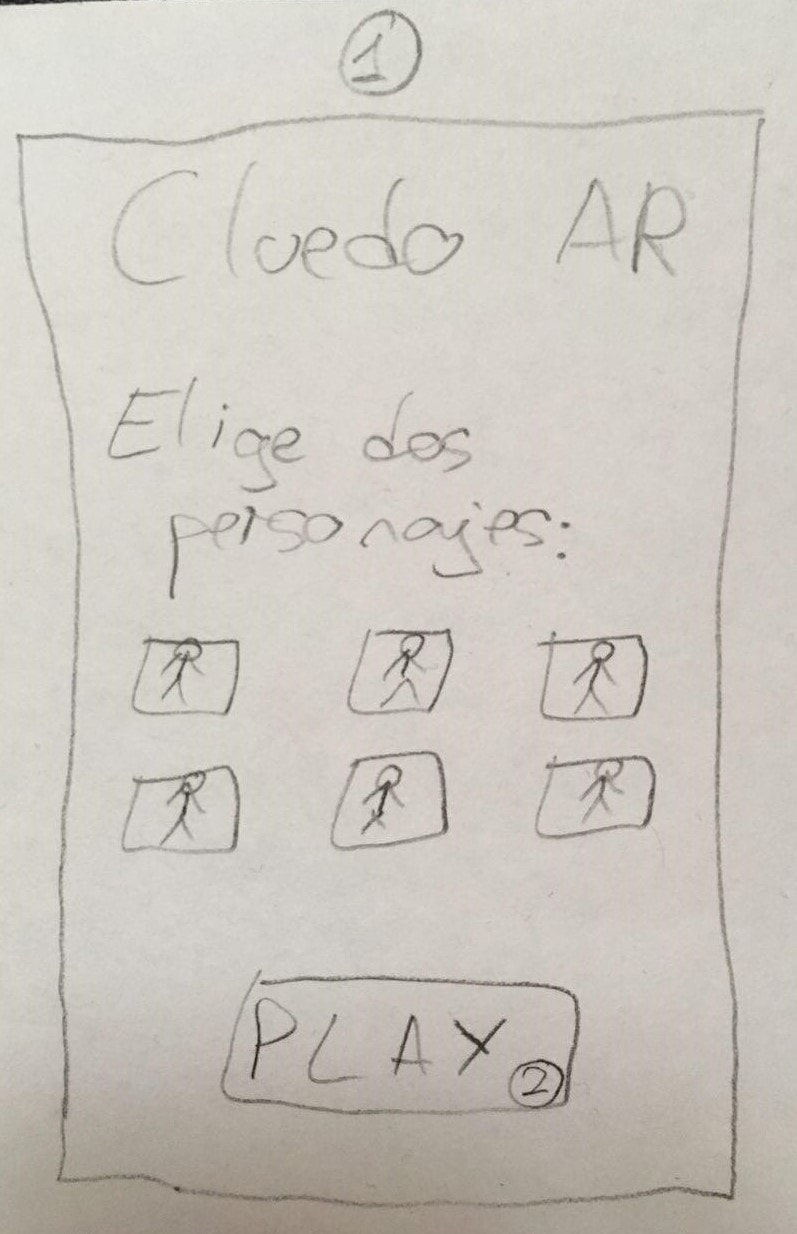
\includegraphics[height=3.5in]{b1.jpg}}
  \qquad
  \subfigure{
  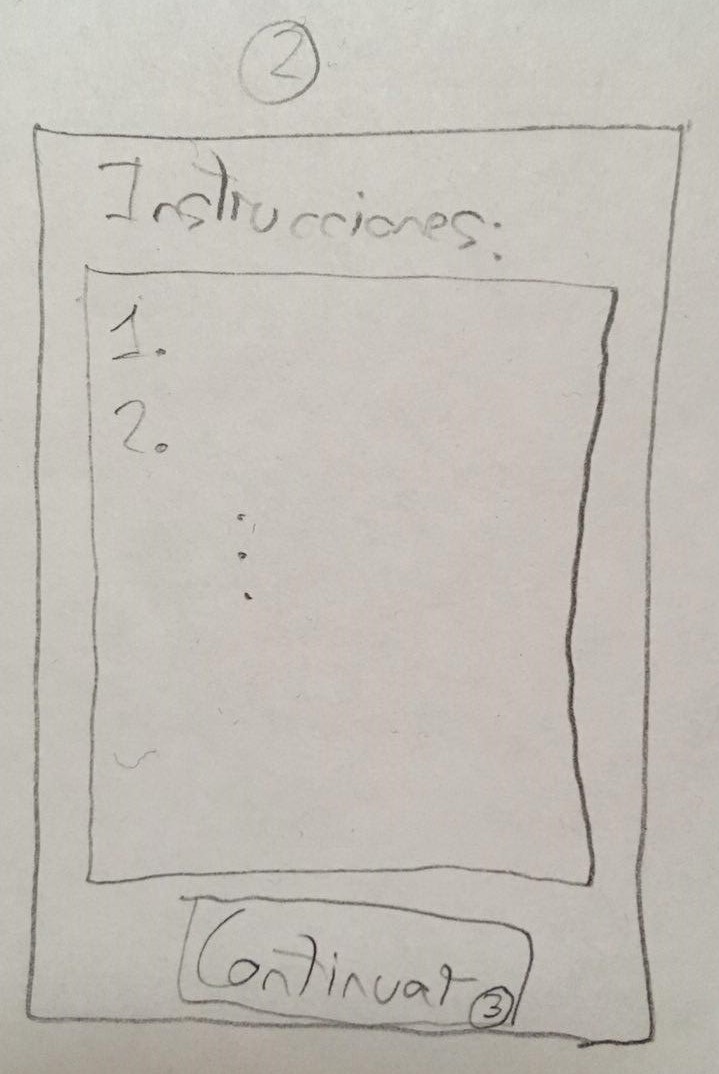
\includegraphics[height=3.5in]{b2.jpg}}
\end{figure}

\newpage

Bocetos sobre la pantalla de juego, con diferentes visualizaciones:

\begin{figure}[h]
  \subfigure{
  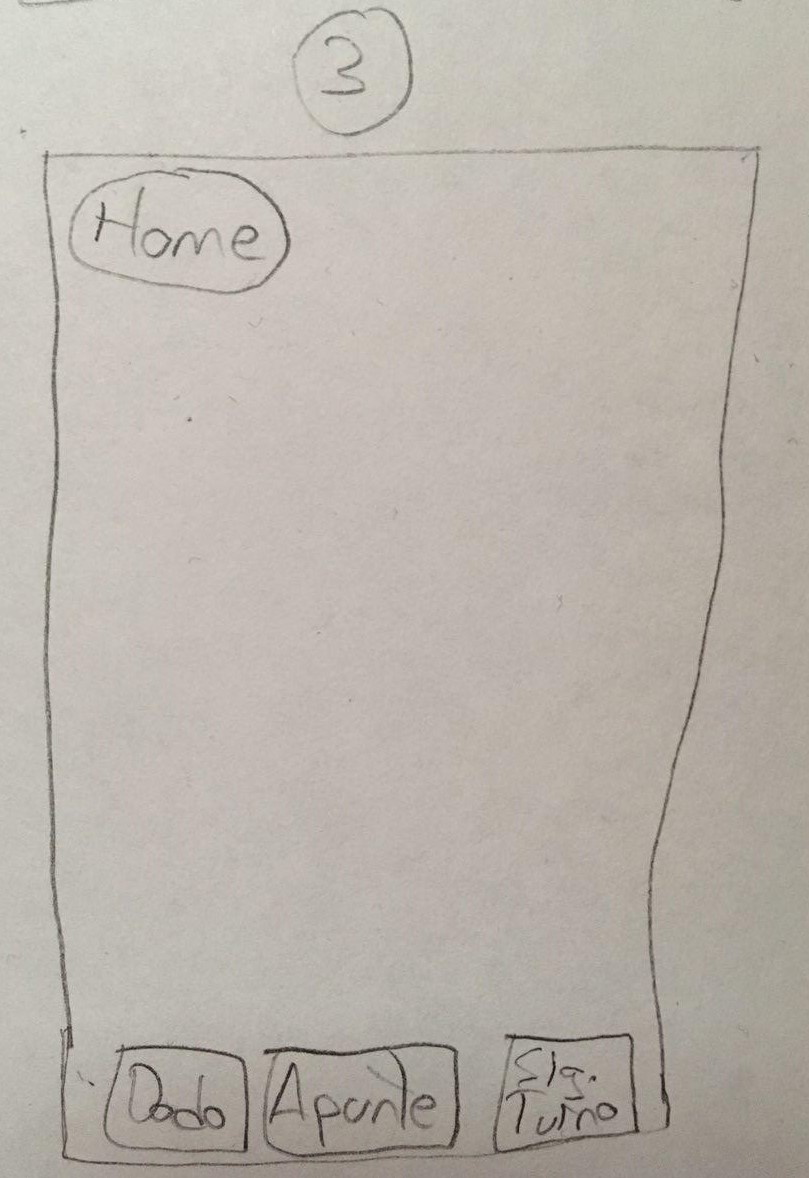
\includegraphics[height=3.05in]{b3.jpg}}
  \qquad
  \subfigure{
  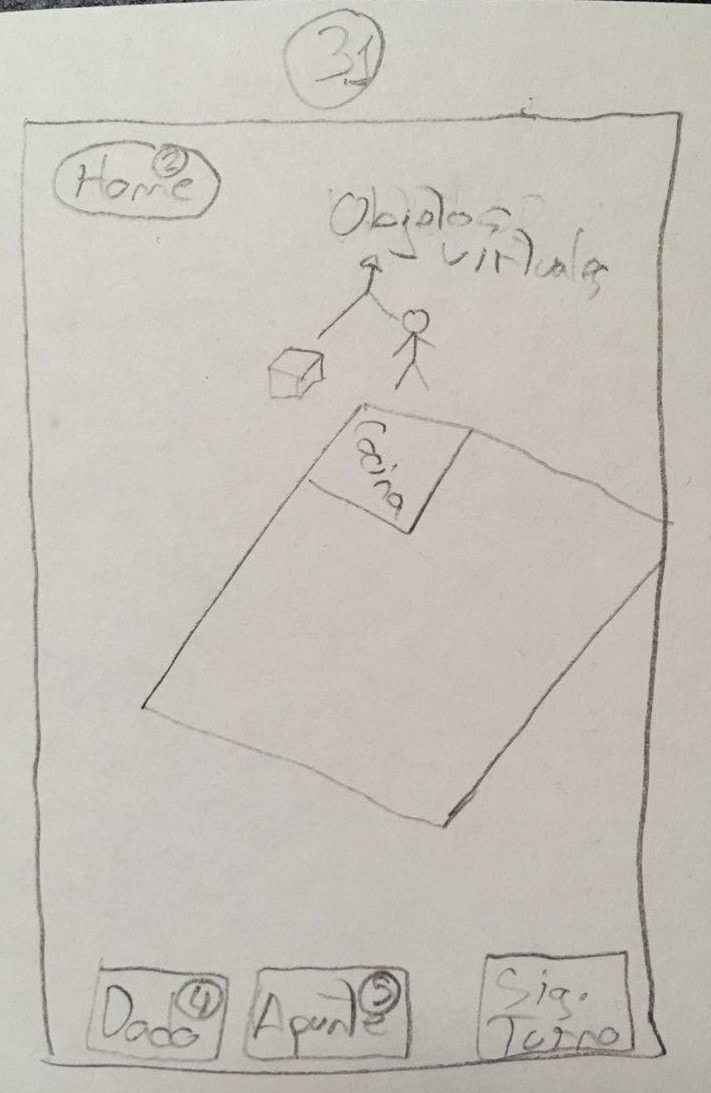
\includegraphics[height=3.1in]{b3-1.jpg}}
\end{figure}

Bocetos sobre la pantalla de juego, y la de selección de habitación:

\begin{figure}[h]
  \centering
  \subfigure{
  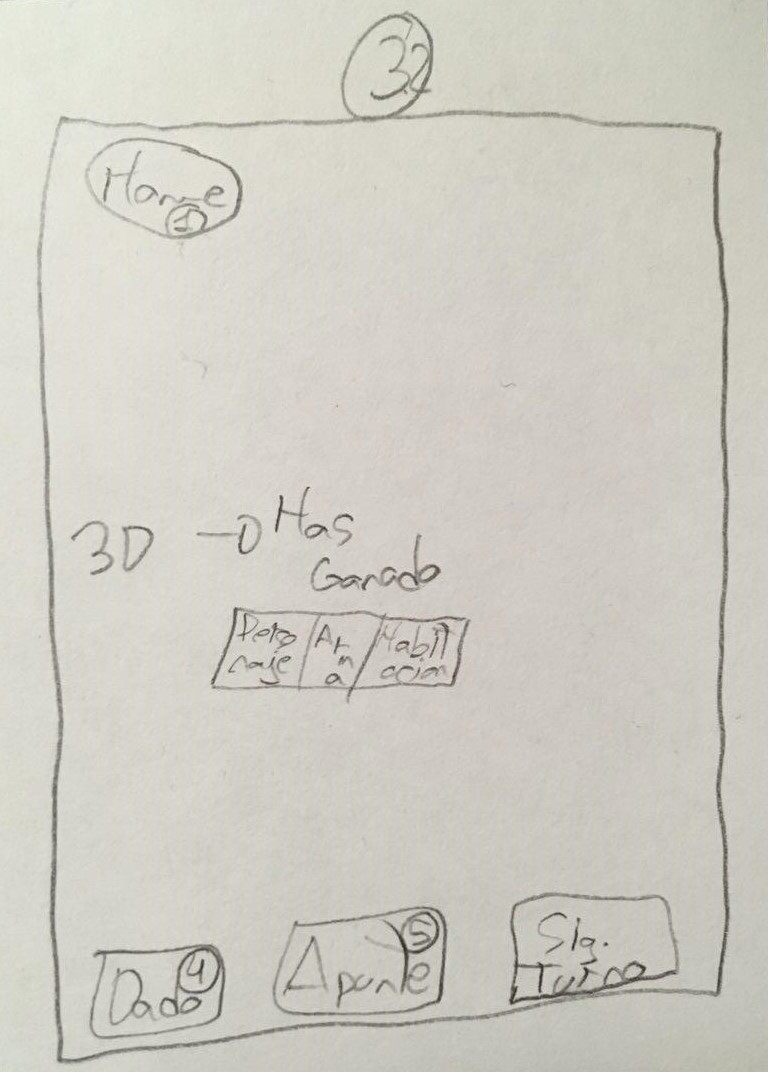
\includegraphics[height=2.95in]{b3-2.jpg}}
  \qquad
  \subfigure{
  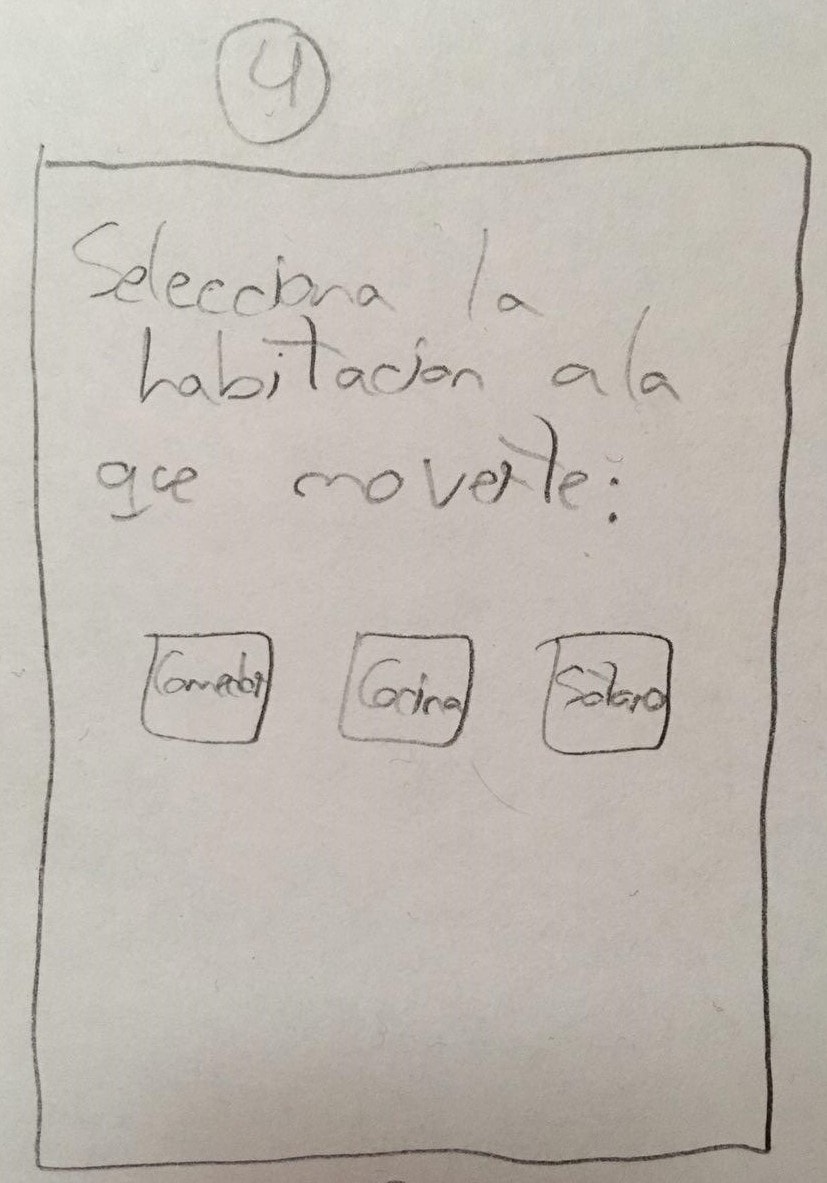
\includegraphics[height=2.95in]{b4.jpg}}
\end{figure}

\newpage

Bocetos sobre la pantalla de tomar apuntes y la pantalla cuando un jugador gana el juego:

\begin{figure}[h]
  \centering
  \subfigure{
  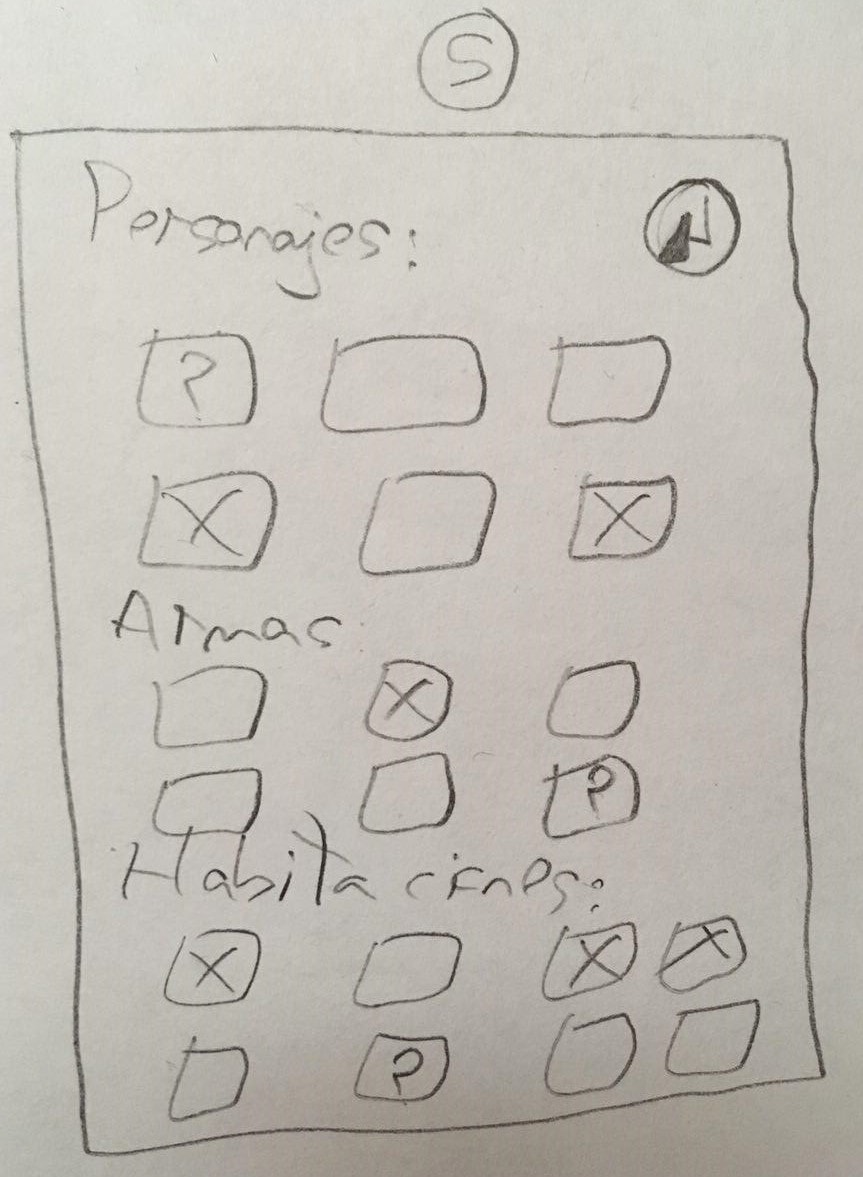
\includegraphics[height=3in]{b5.jpg}}
  \qquad
  \subfigure{
  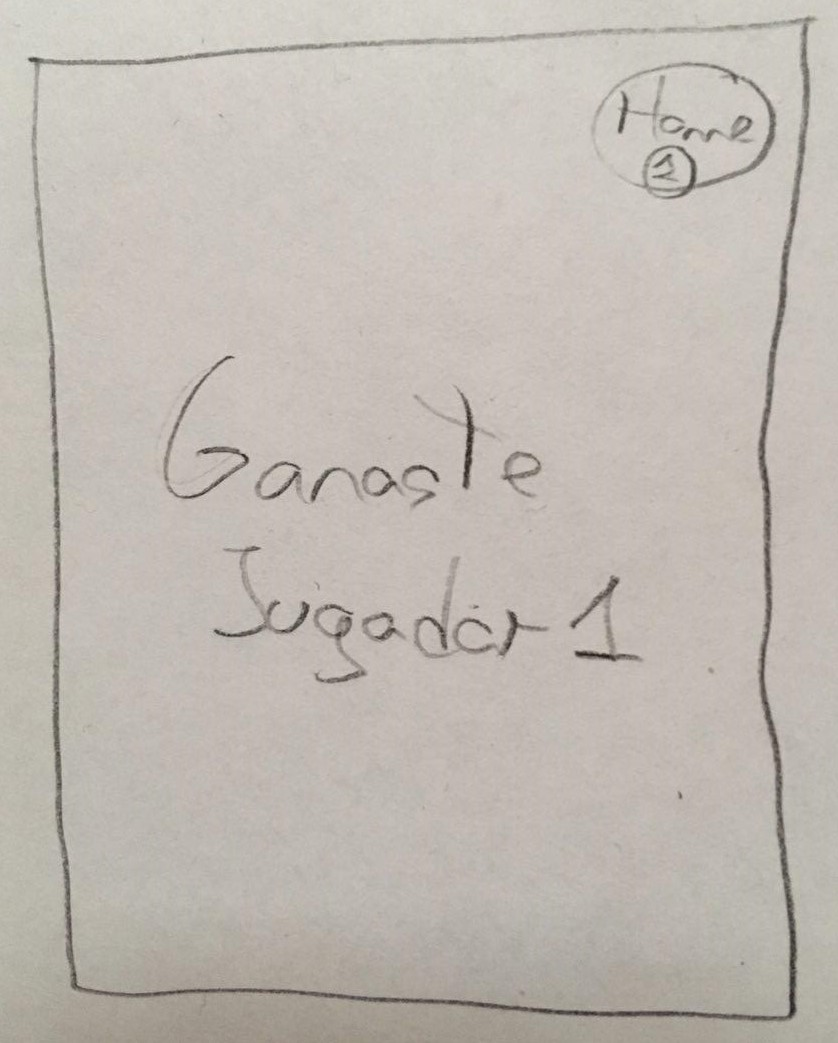
\includegraphics[height=3in]{b6.jpg}}
\end{figure}

%%%%%%%%%%%%%%%%%%%%%%%%%%%%%%%%%%%%%%%%%%%%%%%%%%%%%% TABLAS USABILIDAD %%%%%%%%%%%%%%%%%%%%%%%%%%%%%%%%%%%%%%%%%%%%%%%%%%%%%%

\section{Tablas de usabilidad para los bocetos} \label{tablas-usabilidad-bocetos}

\begin{table}
  \begin{center}
    \begin{tabular}{|p{2.5cm}|p{1.75cm}|p{1.25cm}|p{1.25cm}|p{2.75cm}|p{3.5cm}|}

      \hline
        \rowcolor{Gray} \textbf{Escenario de uso}
        & \textbf{Tarea}
        & \textbf{Éxito/ Fracaso}
        & \textbf{Tiempo}
        & \textbf{Dificultades encontradas}
        & \textbf{Comentarios}\\

      \hline
      El usuario se encuentra jugando una partida
      & Seleccionar ajustes iniciales
      & Éxito
      & 10 seg
      & Le cuesta seleccionar el personaje con el dedo
      & Hacer los botones de personaje mas grandes para facilitar a los usuarios este proceso\\

      \hline
      El usuario se encuentra jugando una partida
      & Comenzar el juego
      & Éxito
      & 5 seg
      & Ninguna
      &\\

      \hline
      El usuario se encuentra jugando una partida
      & Salir de las instrucciones
      & Éxito
      & 5 seg
      & Ninguna
      &\\

      \hline
      El usuario se encuentra jugando una partida
      & Escanear el tablero
      & Éxito
      & 10 seg
      & Ninguna
      &\\

      \hline
      El usuario se encuentra jugando una partida
      & Lanzar el dado
      & Éxito
      & 20 seg
      & Ninguna
      & Añadir imagen con el nombre de la habitación para facilitar a los usuarios este proceso\\

      \hline
      El usuario se encuentra jugando una partida
      & Hacer apunte
      & Éxito
      & 25 seg
      & Ninguna
      &\\

      \hline
      El usuario se encuentra jugando una partida
      & Escanear acusación
      & Éxito
      & 20 seg
      & Ninguna
      &\\

      \hline
      El usuario se encuentra jugando una partida
      & Pasar de turno
      & Éxito
      & 5 seg
      & Ninguna
      &\\

      \hline
      El usuario se encuentra jugando una partida
      & Volver a la pantalla inicial
      & Fracaso
      & 15 seg
      & No sabe donde seleccionar terminar partida
      & Cambiar el texto del botón home por Terminar partida\\

      \hline
      El usuario se encuentra jugando una partida
      & Finalizar después de ganar
      & Éxito
      & 5 seg
      & No sabe donde seleccionar para salir de esa pantalla
      & Cambiar el texto del botón home por Continuar\\

      \hline

    \end{tabular}

    \caption{Resultados usabilidad con Usuario 1.}
    \label{tabla-bocetos-usuario1}

  \end{center}
\end{table}


\begin{table}
  \begin{center}
    \begin{tabular}{|p{2.5cm}|p{1.75cm}|p{1.25cm}|p{1.25cm}|p{2.75cm}|p{3.5cm}|}

      \hline
        \rowcolor{Gray} \textbf{Escenario de uso}
        & \textbf{Tarea}
        & \textbf{Éxito/ Fracaso}
        & \textbf{Tiempo}
        & \textbf{Dificultades encontradas}
        & \textbf{Comentarios}\\

      \hline
      El usuario se encuentra jugando una partida
      & Seleccionar ajustes iniciales
      & Éxito
      & 5 seg
      & Ninguna
      &\\

      \hline
      El usuario se encuentra jugando una partida
      & Comenzar el juego
      & Éxito
      & 5 seg
      & Ninguna
      &\\

      \hline
      El usuario se encuentra jugando una partida
      & Salir de las instrucciones
      & Éxito
      & 5 seg
      & Ninguna
      &\\

      \hline
      El usuario se encuentra jugando una partida
      & Escanear el tablero
      & Éxito
      & 15 seg
      & Ninguna
      &\\

      \hline
      El usuario se encuentra jugando una partida
      & Lanzar el dado
      & Éxito
      & 10 seg
      & Ninguna
      & \\

      \hline
      El usuario se encuentra jugando una partida
      & Hacer apunte
      & Fracaso
      & 25 seg
      & No comprendía el funcionamiento de cómo realizar un apunte
      & Explicar en la pantalla de instrucciones inicial como se realiza un apunte\\

      \hline
      El usuario se encuentra jugando una partida
      & Escanear acusación
      & Éxito
      & 10 seg
      & Ninguna
      &\\

      \hline
      El usuario se encuentra jugando una partida
      & Pasar de turno
      & Éxito
      & 3 seg
      & Ninguna
      &\\

      \hline
      El usuario se encuentra jugando una partida
      & Volver a la pantalla inicial
      & Fracaso
      & 7 seg
      & No encontraba el botón de inicio
      & Cambiar el texto del botón a español y mas grande\\

      \hline
      El usuario se encuentra jugando una partida
      & Finalizar después de ganar
      & Éxito
      & 3 seg
      & No sabe que significa home, el botón es pequeño y poco accesible
      & Cambiar el texto del botón a español y mas grande\\

      \hline

    \end{tabular}

    \caption{Resultados usabilidad con Usuario 2.}
    \label{tabla-bocetos-usuario2}

  \end{center}
\end{table}


\begin{table}
  \begin{center}
    \begin{tabular}{|p{2.5cm}|p{1.75cm}|p{1.25cm}|p{1.25cm}|p{2.75cm}|p{3.5cm}|}

      \hline
        \rowcolor{Gray} \textbf{Escenario de uso}
        & \textbf{Tarea}
        & \textbf{Éxito/ Fracaso}
        & \textbf{Tiempo}
        & \textbf{Dificultades encontradas}
        & \textbf{Comentarios}\\

      \hline
      El usuario se encuentra jugando una partida
      & Seleccionar ajustes iniciales
      & Éxito
      & 5 seg
      & Ninguna
      & Activar el botón de play cuando haya seleccionado 2 personajes\\

      \hline
      El usuario se encuentra jugando una partida
      & Comenzar el juego
      & Éxito
      & 5 seg
      & Ninguna
      &\\

      \hline
      El usuario se encuentra jugando una partida
      & Salir de las instrucciones
      & Éxito
      & 5 seg
      & Ninguna
      &\\

      \hline
      El usuario se encuentra jugando una partida
      & Escanear el tablero
      & Éxito
      & 3 seg
      & Ninguna
      &\\

      \hline
      El usuario se encuentra jugando una partida
      & Lanzar el dado
      & Éxito
      & 15 seg
      & El botón de dado no era muy descriptivo y el usuario no sabia si ahí se lanzaba
      & Cambiar el texto del botón dado a Lanzar dado\\

      \hline
      El usuario se encuentra jugando una partida
      & Hacer apunte
      & Éxito
      & 20 seg
      & El botón usuario no entiende que pasa al pulsar el botón de apunte
      & Cambiar el texto del botón de apunte a Notas\\

      \hline
      El usuario se encuentra jugando una partida
      & Escanear acusación
      & Éxito
      & 10 seg
      & Ninguna
      &\\

      \hline
      El usuario se encuentra jugando una partida
      & Pasar de turno
      & Éxito
      & 3 seg
      & Ninguna
      &\\

      \hline
      El usuario se encuentra jugando una partida
      & Volver a la pantalla inicial
      & Éxito
      & 3 seg
      & Ninguna
      &\\

      \hline
      El usuario se encuentra jugando una partida
      & Finalizar después de ganar
      & Éxito
      & 3 seg
      & Ninguna
      & Camiar el texto a Continuar y cambiar su posición y tamaño\\

      \hline

    \end{tabular}

    \caption{Resultados usabilidad con Usuario 3.}
    \label{tabla-bocetos-usuario3}

  \end{center}
\end{table}

\end{itemize}

\FloatBarrier

%%%%%%%%%%%%%%%%%%%%%%%%%%%%%%%%%%%%%%%%%%% ESTUDIO DE MERCADO APPS AR %%%%%%%%%%%%%%%%%%%%%%%%%%%%%%%%%%%%%%%%%%%%%%%%%

\section{Estudio de mercado sobre aplicaciones que hacen uso de realidad aumentada}

Este estudio de mercado explora los diferentes usos que se da a la realidad aumentada en aplicaciones actualmente, por lo que se listarán los tipos de uso:

\begin{itemize}
  \item \textbf{Puzzle-Perspectiva}: Consisten en puzles que se resuelven utilizando la perspectiva, moviéndote alrededor del puzle que se m uestra en 3D sobre una superficie plana.
  \begin{itemize}
    \item \textbf{Mazelith}: Este juego ha utilizado el 3D para que en función del lugar desde el que visualices la pieza se pueda resolver el puzle, uniendo la vía por la que circula la luz. La ventaja que le da la realidad aumentada a este juego es el aumento de realismo, ya que ahora lo juegas físicamente moviéndote alrededor en lugar de mover la escena con los dedos para encontrar la perspectiva adecuada.

    \begin{figure}[h]
      \centering
      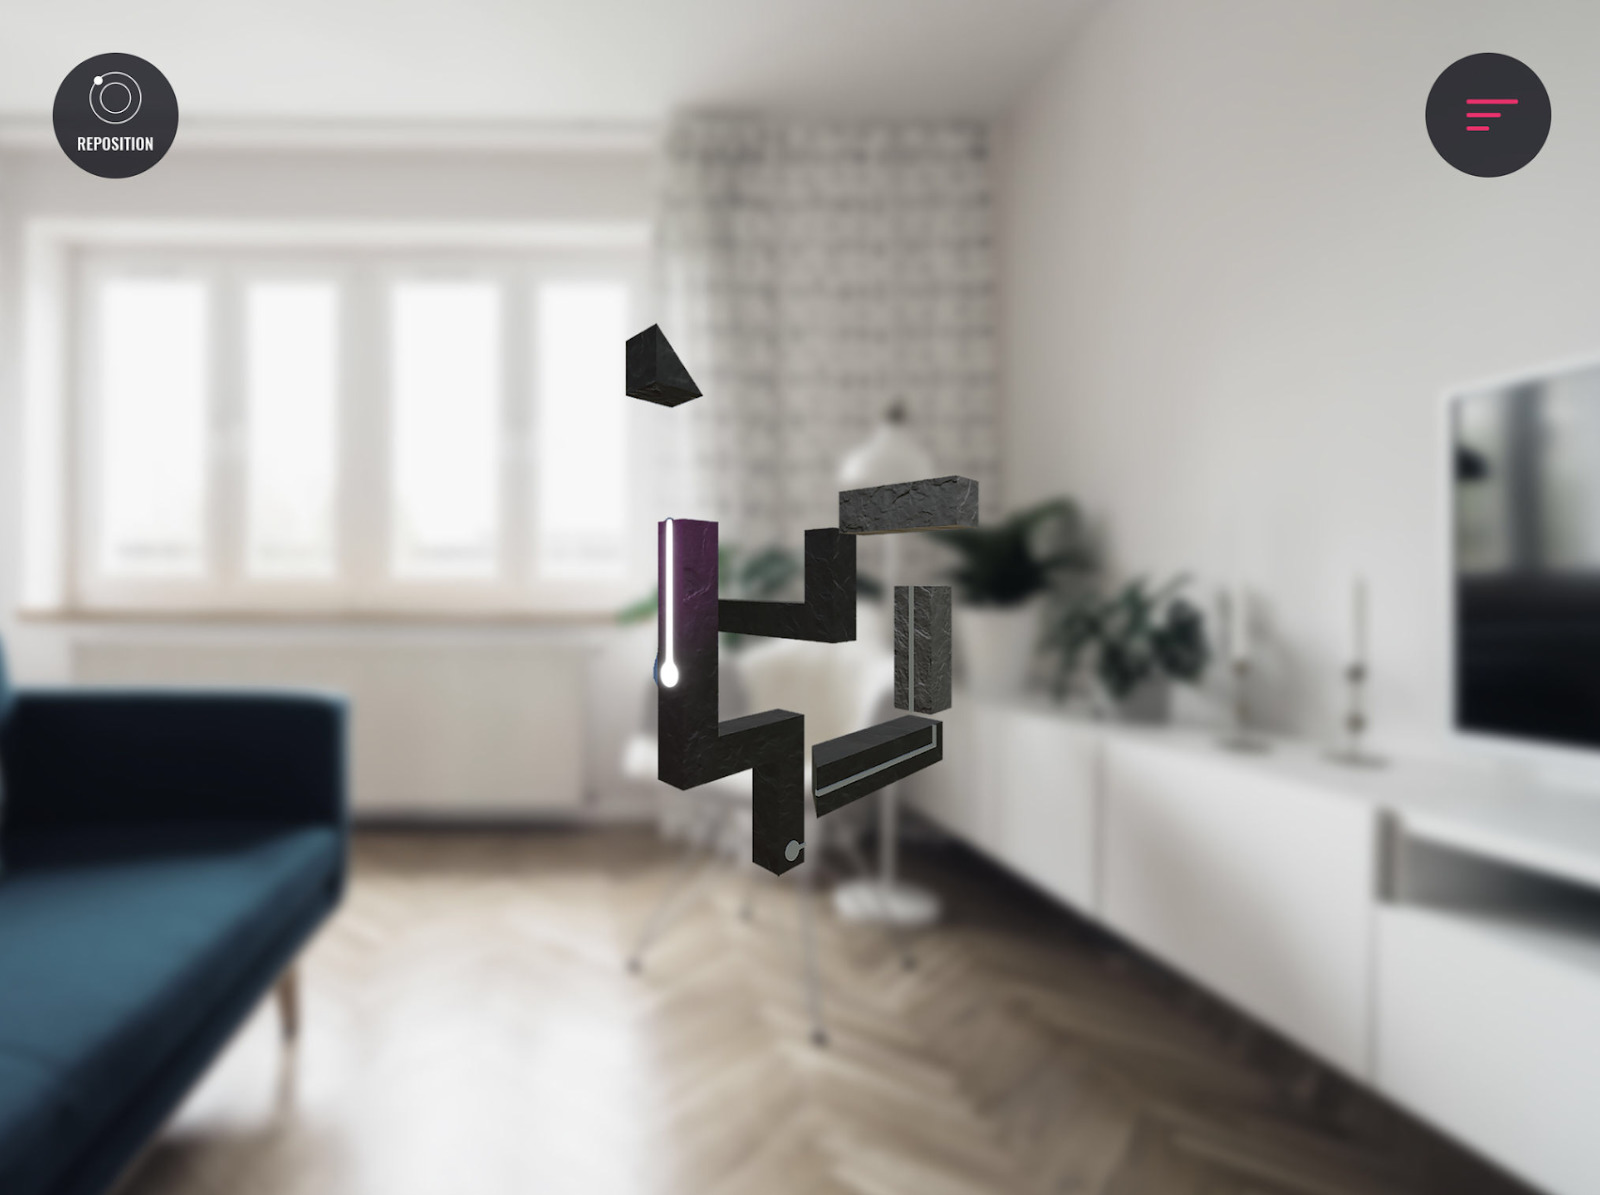
\includegraphics[scale=0.13]{mazelith}
      \caption{Imagen que muestra el juego Mazelith.\protect\footnotemark}
      \label{figura-mazelith}
    \end{figure}

    \footnotetext{ \url{https://itunes.apple.com/es/app/mazelith/id1328826457?mt=8}, Monogrid}
  \end{itemize}

  \item \textbf{Shooter}: Consisten en enemigos virtuales que se muestran en el espacio físico de tu alrededor, a los cuales tienes que disparar para conseguir más puntuación.

  \begin{itemize}
    \item \textbf{Ghosts’n guns - AR Shooter}: Este juego utiliza el concepto de shooter clásico, en el que te aparecen enemigos y tienes que dispararles hasta derrotarlos. Utiliza la realidad aumentada de forma que ahora en lugar de estar todo dentro de la pantalla, tu eres el que dispara en la vida real y tienes que apuntar con el móvil bien para acertar, introduciendo un mayor realismo en el juego.

    \begin{figure}[h]
      \centering
      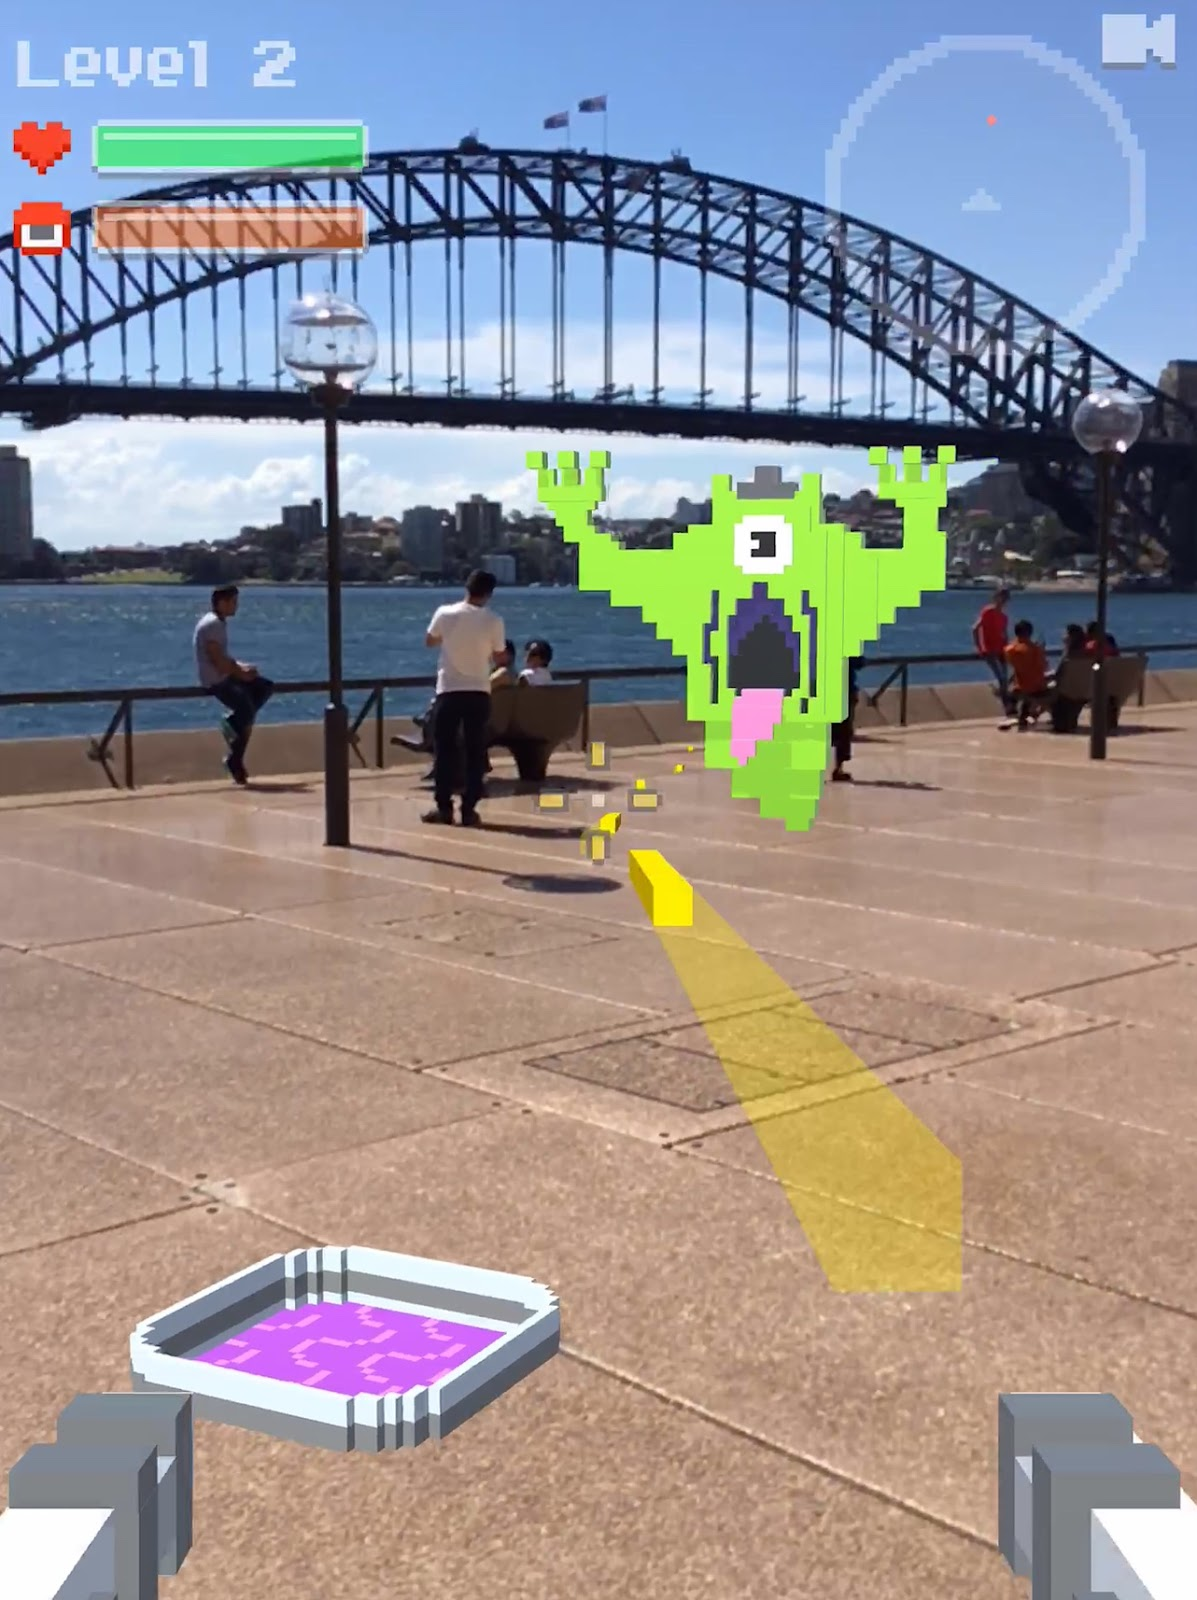
\includegraphics[scale=0.12]{ghostsguns}
      \caption{Imagen que muestra el juego Ghosts'n guns.\protect\footnotemark}
      \label{figura-ghosts-guns}
    \end{figure}

    \footnotetext{ \url{https://itunes.apple.com/us/app/ghosts-n-guns-ar/id1312708394?mt=8}, Turbo Chilli Pty Ltd}
  \end{itemize}

  \item \textbf{Mapa 3D}: Consisten en juegos que sitúan un mapa sobre una superficie plana, y la dinámica del juego es la misma que si fuera en 2D en la pantalla, pero ahora recibes nuevas perspectivas en 3D.

  \begin{itemize}
    \item \textbf{Siege Breakers}: Este juego consiste en demoler edificios colocando explosivos estratégicamente. La aplicación de realidad aumentada en este caso permite una mejor experiencia de usuario, ya que resulta más sencillo moverse alrededor del edificio y por tanto la decisión de dónde colocar el explosivo será más sencilla y efectiva.

    \begin{figure}[h]
      \centering
      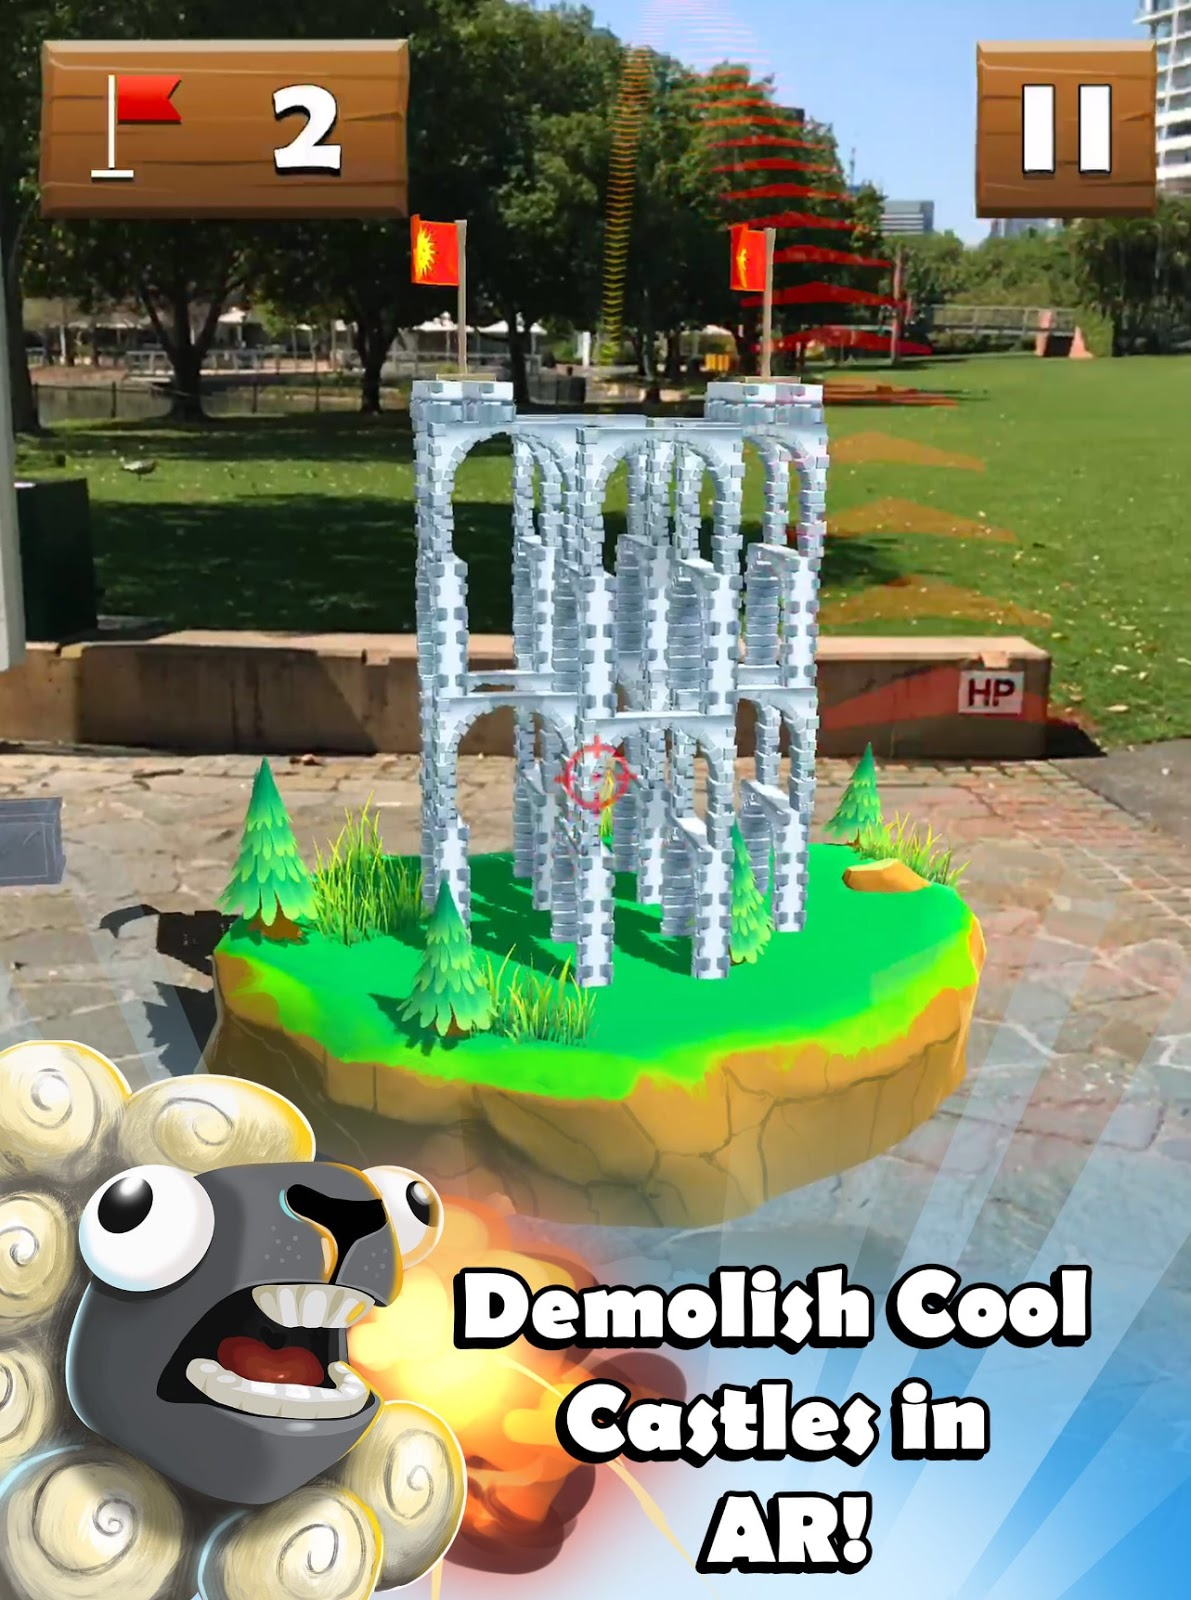
\includegraphics[scale=0.1]{siegebreakers}
      \caption{Imagen que muestra el juego Siege Breakers.\protect\footnotemark}
      \label{figura-siege-breakers}
    \end{figure}

    \footnotetext{ \url{https://itunes.apple.com/es/app/siege-breakers/id1276405526?mt=8}, Halfbrick Studios}
  \end{itemize}

  \newpage

  \item \textbf{Juegos de mesa}: Consisten en un juego de mesa, que en lugar de mostrarse en la pantalla, se sitúa en una superficie plana, por ejemplo una mesa, dando una sensación de jugar un juego de mesa real.

  \begin{itemize}
    \item \textbf{Chess+ AR}: Este juego consiste en situar un tablero de ajedrez en una superficie plana del mundo real, y jugar una partida de ajedrez. La realidad aumentada permite situar el tablero en el mundo real, dando la sensación de ser un juego real, aunque físicamente no esté.

    \begin{figure}[h]
      \centering
      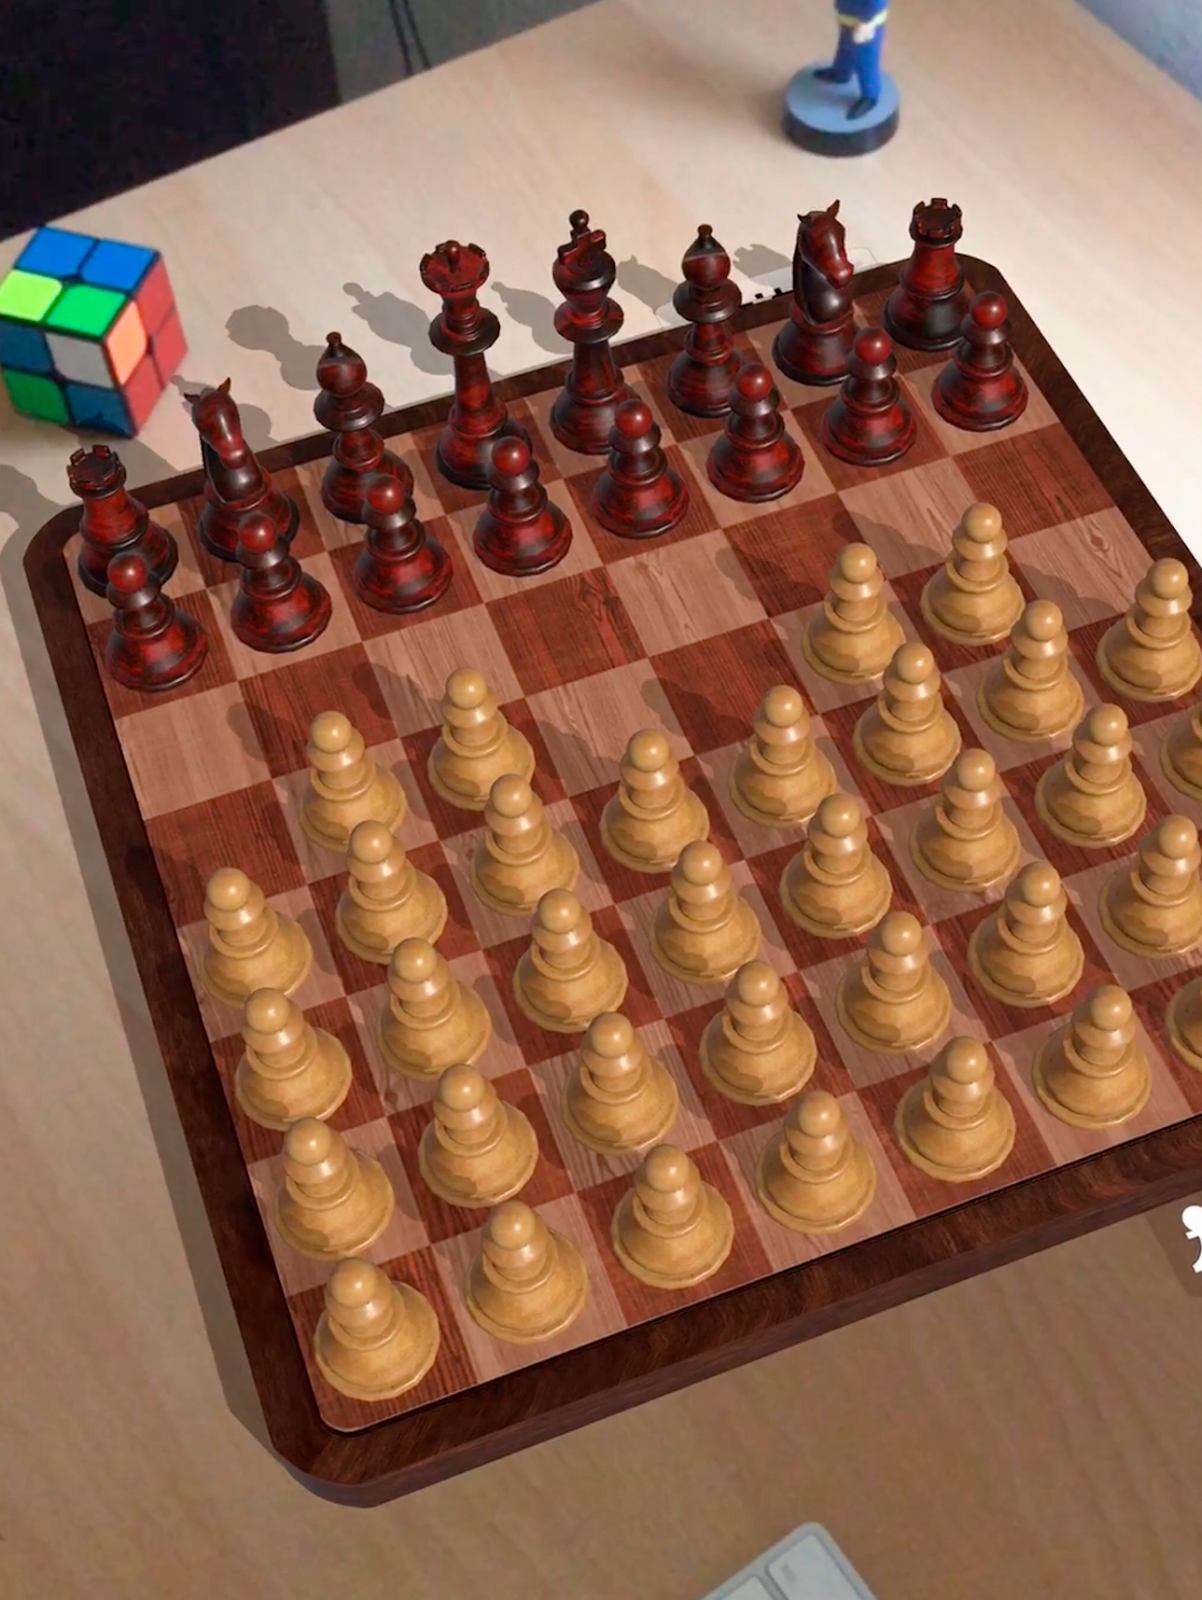
\includegraphics[scale=0.1]{chess}
      \caption{Imagen que muestra el juego Chess+ AR.\protect\footnotemark}
      \label{figura-siege-breakers}
    \end{figure}

    \footnotetext{ \url{https://itunes.apple.com/us/app/chess-ar/id1273831380?mt=8}, Jorge Moreno Aguilera}
  \end{itemize}

  \newpage

  \item \textbf{Exploración}: Consisten en aprovechar el conocimiento de la posición del dispositivo en el entorno físico, y que se almacena todas las superficies a tu alrededor, de forma que se aprovechan todas estas superficies registradas, por ejemplo, enterrando cofres del tesoro, y en el siguiente turno el otro jugador tiene que desenterrarlos.

  \begin{itemize}
    \item \textbf{AR Runner}: Ese juego consiste en recorrer un circuito físicamente, va mostrando puntos y tienes que situarte sobre estos para completar esa parte del circuito. La realidad aumentada igual que en el caso anterior permite algo que hasta ahora no existía, y es convertir el mundo real en el mapa de juego.

    \begin{figure}[h]
      \centering
      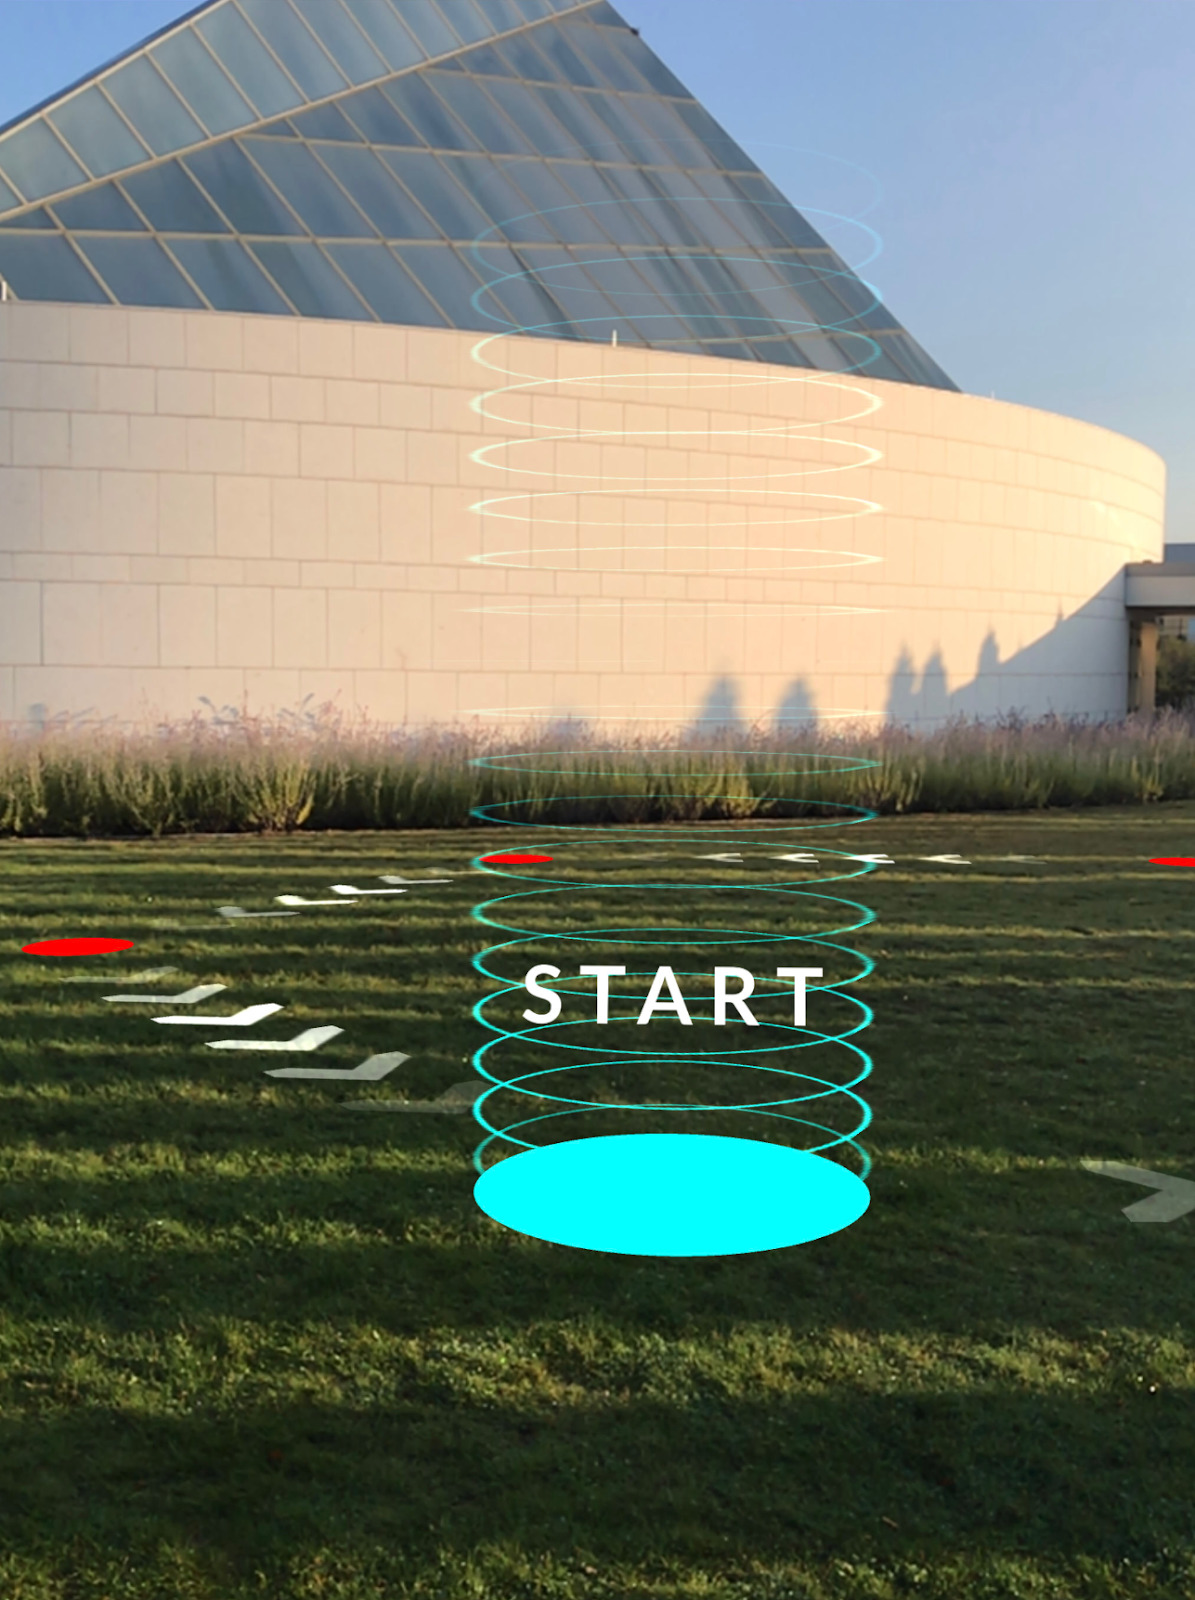
\includegraphics[scale=0.1]{arrunner}
      \caption{Imagen que muestra el juego AR Runner.\protect\footnotemark}
      \label{figura-ar-runner}
    \end{figure}

    \footnotetext{ \url{https://itunes.apple.com/us/app/ar-runner/id1275938861?mt=8}, Semidome Inc.}
  \end{itemize}

  \item \textbf{Astronomía}: Consisten en mostrarnos las constelaciones y elementos del universo basado en nuestra geolocalización, y estos se muestran sobre lo que la cámara recibe, es decir si quieres ver las constelaciones por la noche apuntas con la cámara y te indica donde estas están y te las muestra facilitando su visualización y localización.

  \begin{itemize}
    \item \textbf{Night Sky}: Esta aplicación consiste en visualizar las constelaciones, satélites y más elementos del universo, mostrandote donde se encuentran cada uno de los elementos para facilitar al usuario su visualización. La realidad aumentada aporta una mejor experiencia de usuario, al facilitar el proceso de encontrar donde se sitúan estos elementos, ya que al mostrar sobre lo que percibe la cámara es más fácil para el usuario localizarlo.

    \begin{figure}[h]
      \centering
      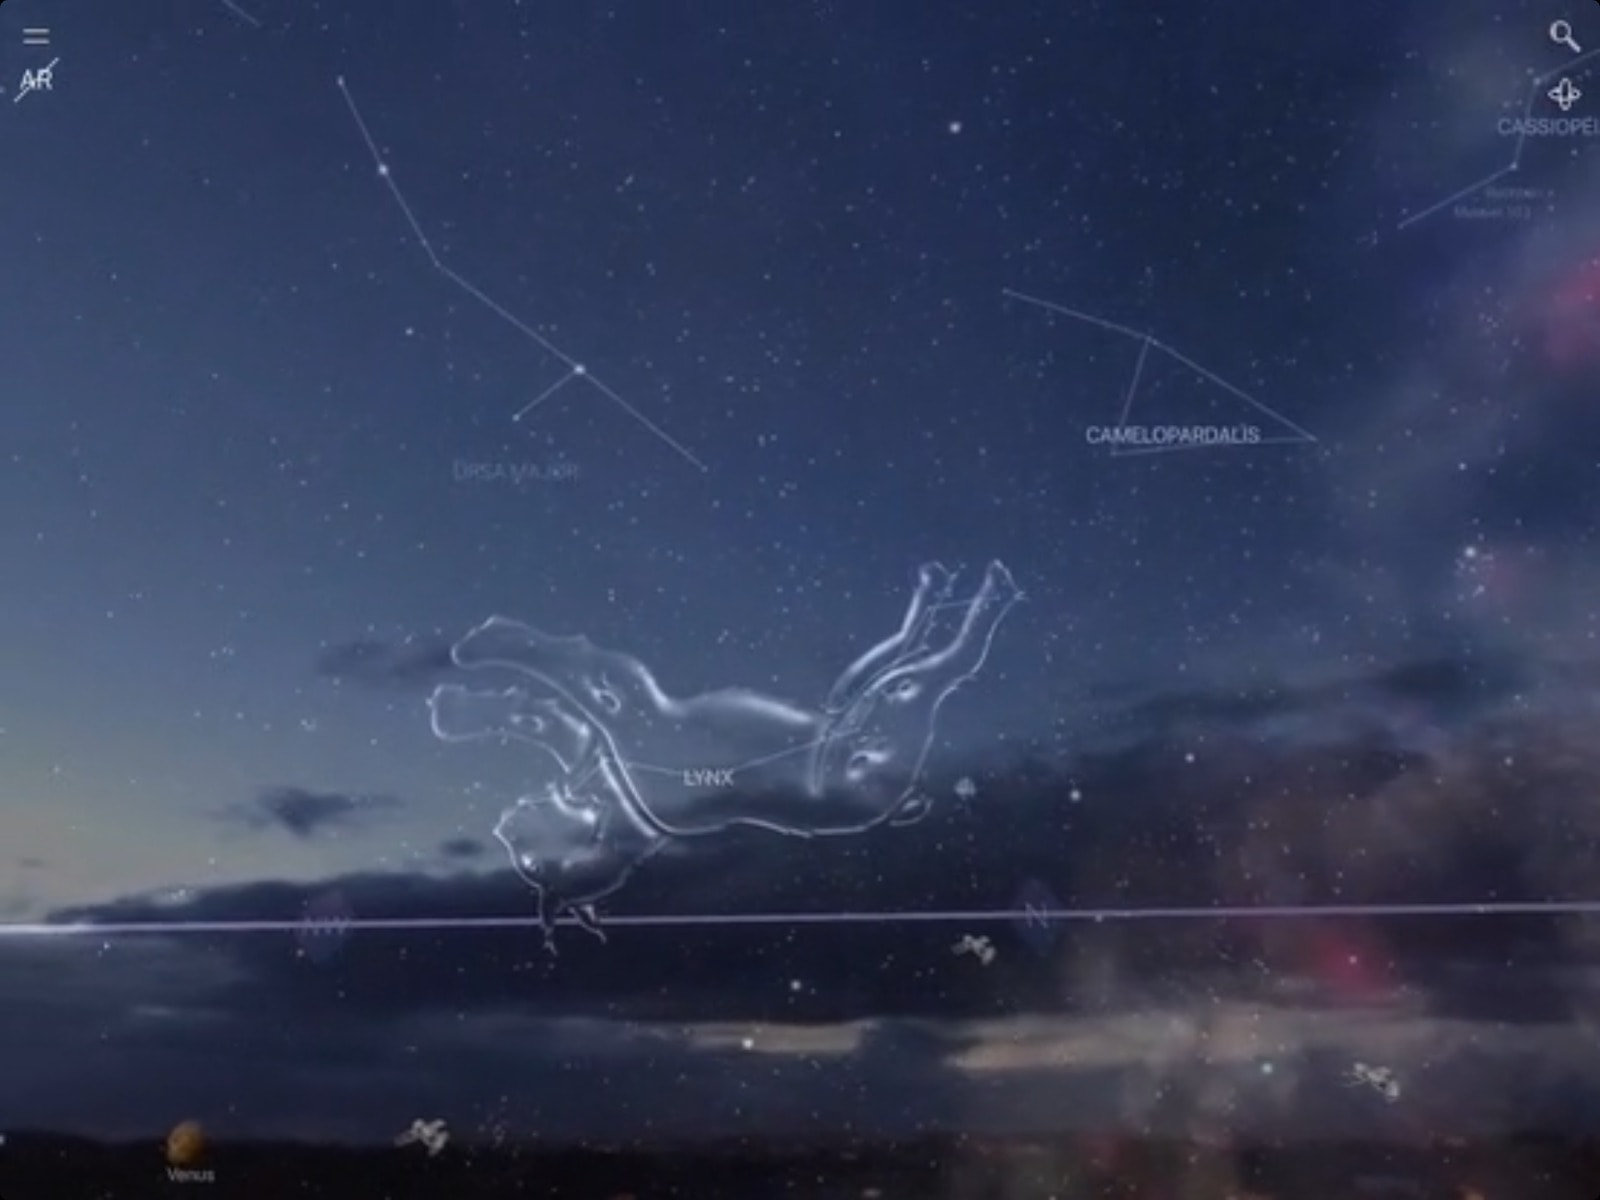
\includegraphics[scale=0.12]{nightsky}
      \caption{Imagen que muestra la aplicación Night Sky.\protect\footnotemark}
      \label{figura-night-sky}
    \end{figure}

    \footnotetext{ \url{https://itunes.apple.com/es/app/night-sky/id475772902?mt=8}, iCandi Apps}
  \end{itemize}

  \item \textbf{Utilidades}: Permiten al usuario llevar a cabo varias tareas que antes eran más difíciles de realizar o para las que necesitabas un dispositivo especial para realizarlas, y que ahora se pueden hacer solamente con tu un smartphone.

  \begin{itemize}
    \item \textbf{AR MeasureKit}: Esta aplicación permite realizar mediciones en el mundo real utilizando solo la camara. La realidad aumentada permite en este caso realizar una tarea que antes era imposible si no disponías de algún dispositivo de medida.

    \begin{figure}[h]
      \centering
      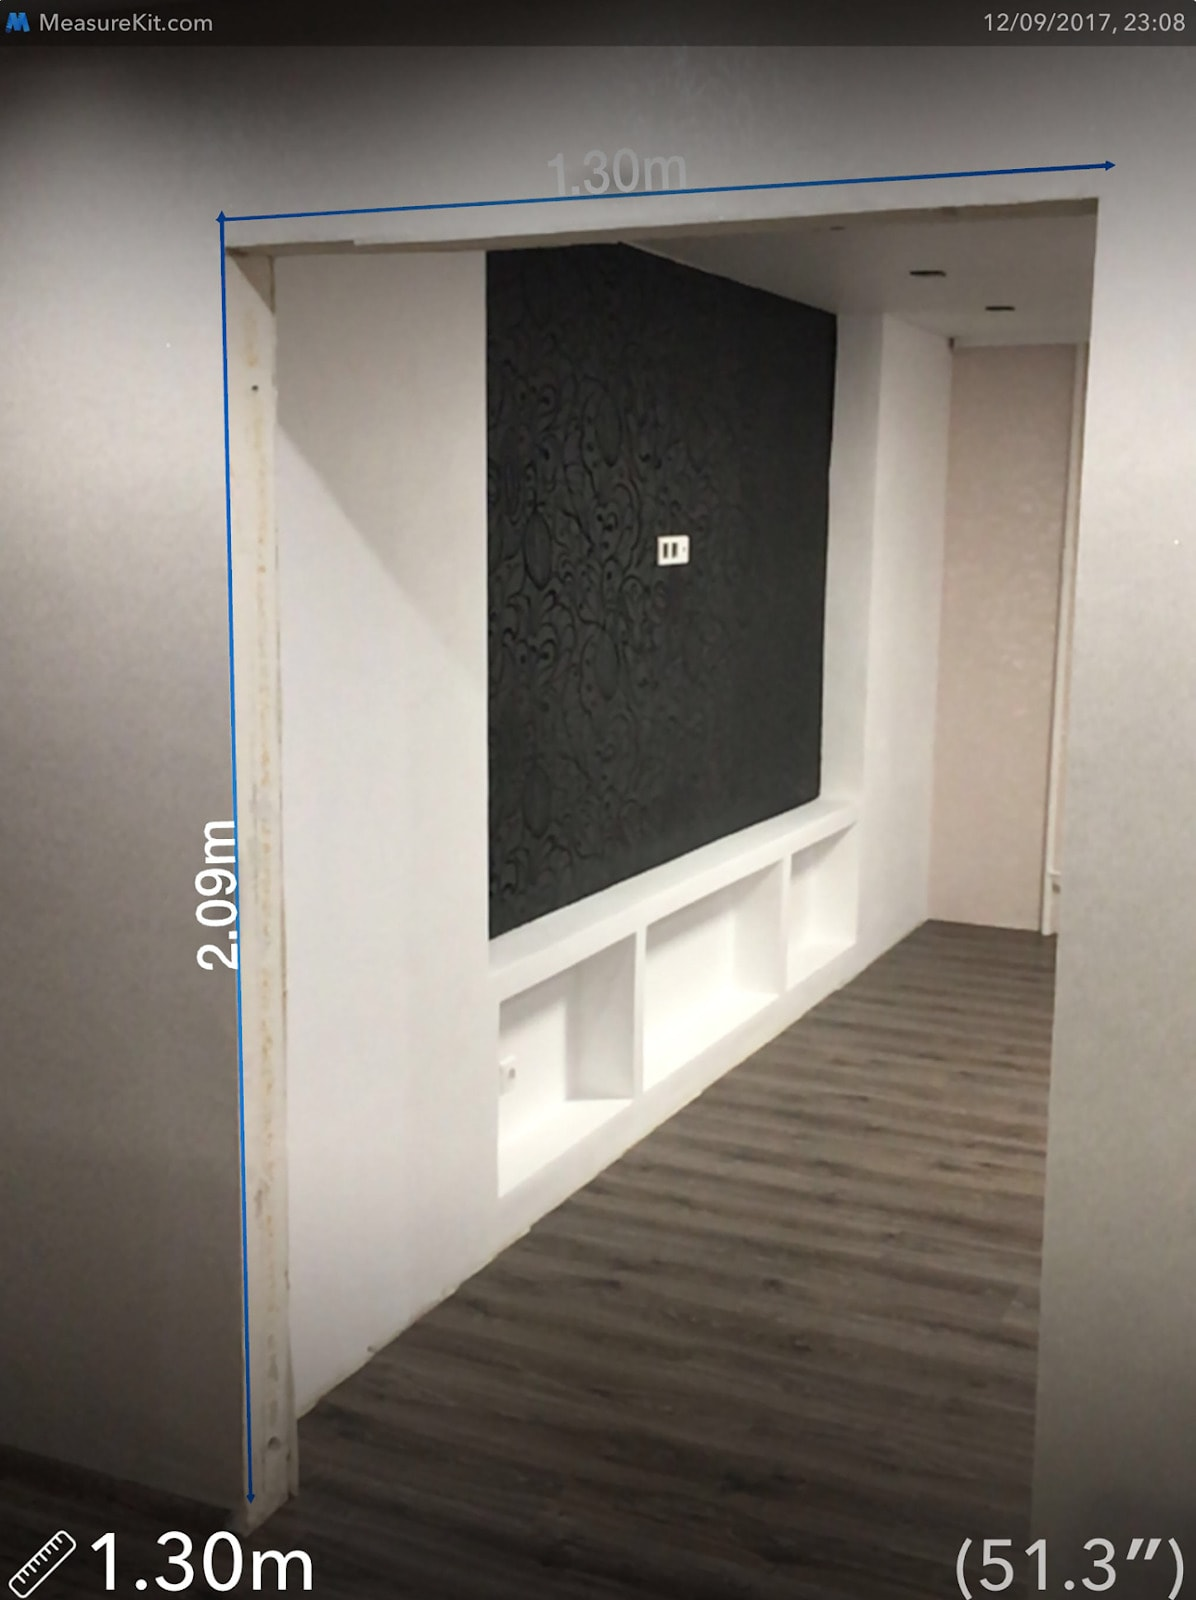
\includegraphics[scale=0.12]{armeasurekit}
      \caption{Imagen que muestra la aplicación AR MeasureKit.\protect\footnotemark}
      \label{figura-ar-measurekit}
    \end{figure}

    \footnotetext{ \url{https://itunes.apple.com/es/app/ar-measurekit/id1258270451?mt=8}, Rinat Khanov}
  \end{itemize}

  \item \textbf{Entretenimiento}: La funcionalidad principal es generar el entretenimiento del usuario o la creación de contenido situando elementos virtuales a el entorno físico y después fotografiando o grabando.

  \begin{itemize}
    \item \textbf{Monster Park}: Esta aplicación te permite colocar diferentes dinosaurios en tu propia habitación permitiendote hacer fotos o videos con ellos en la escena. La realidad aumentada permite que fotos con elementos inusuales, como puede ser un dinosaurio, se puedan realizar sin necesidad de photoshop y muchas horas de trabajo, y consiguiendo un mejor resultado.

    \begin{figure}[h]
      \centering
      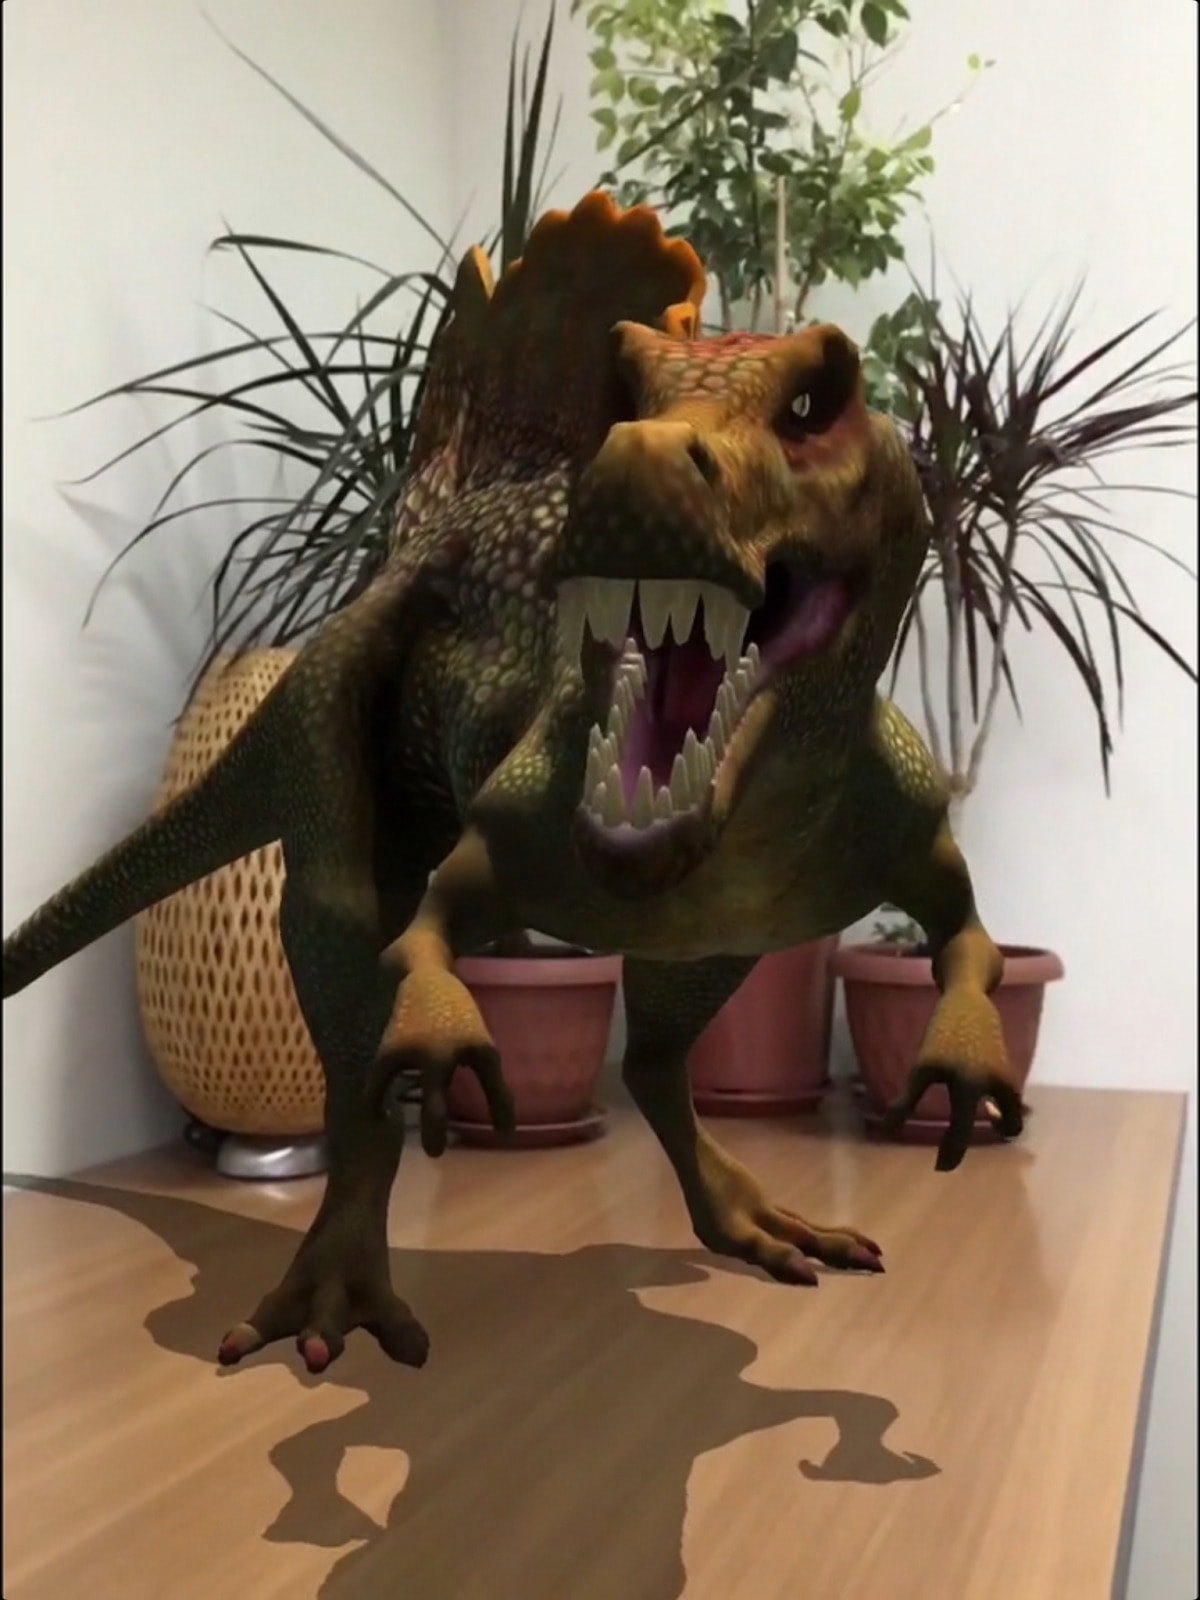
\includegraphics[scale=0.12]{monsterpark}
      \caption{Imagen que muestra la aplicación Monster Park.\protect\footnotemark}
      \label{figura-monster-park}
    \end{figure}

    \footnotetext{ \url{https://itunes.apple.com/es/app/monster-park-mundo-dinosaurio/id1259767702?mt=8}, Vito Technology Inc.}
  \end{itemize}

  \item \textbf{Educación}: Son aplicaciones que tienen un propósito educativo o de compartir conocimientos.

  \begin{itemize}
    \item \textbf{Insight heart}: Es una aplicación que te permite ver en 3D el corazón y sistema circulatorio. La realidad aumentada permite una forma mucho más sencilla, útil e intuitiva de entender el cuerpo humano, ya que al poder explorarlo moviéndote alrededor de este es mucho más natural y puedes ver todo mejor.

    \begin{figure}[h]
      \centering
      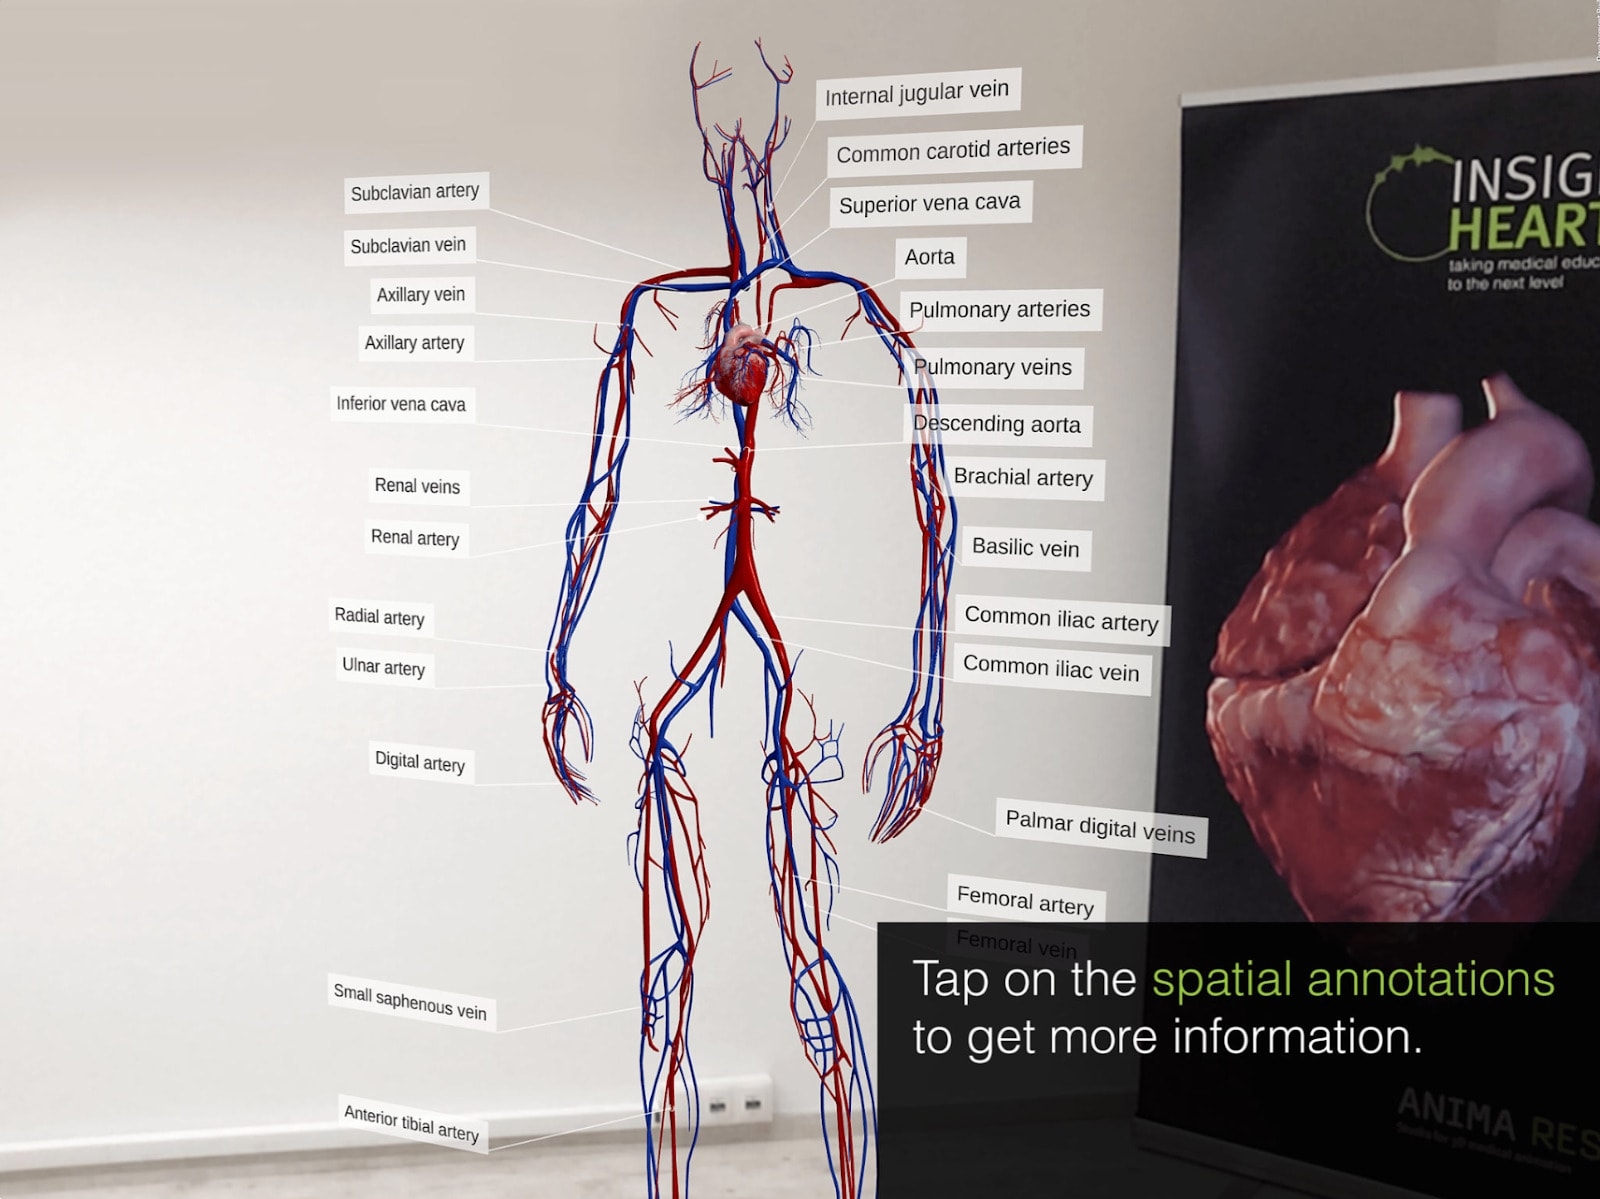
\includegraphics[scale=0.12]{insightheart}
      \caption{Imagen que muestra la aplicación Insight Heart.\protect\footnotemark}
      \label{figura-insight-heart}
    \end{figure}

    \footnotetext{ \url{https://itunes.apple.com/us/app/insight-heart/id1280845473?mt=8}, ANIMA RES}
  \end{itemize}
\end{itemize}

\subsection{Conclusiones}
Como se puede observar en el estudio realizado, la mayoría de aplicaciones y juegos que utilizan realidad aumentada se basan en poner elementos virtuales en el mundo real, pero sin interactuar entre ellos, lo máximo que interactuan es situar información sobre una superficie, por tanto se puede observar la necesidad de juegos con realidad aumentada que utilicen elementos físicos para interactuar dentro de la app, de forma que no toda interacción sea virtual, creando así una experiencia más realista y manteniendo los aportes de la realidad aumentada.
